\documentclass[a4paper,14pt]{extreport} % 14pt шрифт через пакет extsizes
\usepackage[utf8]{inputenc}
\usepackage[T1]{fontenc}
\usepackage{mathtext}
\usepackage[russian]{babel}
\usepackage{geometry} % Меняем поля страницы
\usepackage{wrapfig}
\usepackage{amsmath}
\usepackage{booktabs}
\usepackage{tabularx}
\usepackage[labelsep=period]{caption} % http://ctan.org/pkg/caption%
\usepackage{subcaption} % для subfigure
\usepackage{newunicodechar}
\usepackage{amssymb}
\newunicodechar{∼}{\textasciitilde}
\captionsetup[table]{justification=raggedright,singlelinecheck=off}
\geometry{left=3cm} % левое поле
\geometry{right=2cm} % правое поле
\geometry{top=2cm} % верхнее поле
\geometry{bottom=2cm} % нижнее поле
\setlength{\headheight}{17pt}
\addtolength{\topmargin}{-5pt}
\parindent=1cm % абзацный отступ
\usepackage{indentfirst} % включает отступ для первого абзаца
\linespread{1.3} % полуторный межстрочный интервал
\usepackage{graphicx}
\usepackage{fancyhdr}

\usepackage{svg}
\pagestyle{fancyplain}
\fancyhf{}
\fancyhead[C]{\thepage}
\newcommand{\ket}[1]{|#1\rangle}
\usepackage{titlesec}
\titleformat{\chapter}[hang]{\normalfont\LARGE\bfseries}{\thechapter.}{1em}{}
\titlespacing*{\chapter}{0pt}{-20pt}{10pt}
\begin{document}
\begin{titlepage}
\begin{center}{\bfseries}
\large Феральное государственное бюджетное общеобразовательное учреждение высшего образования<< Московский государственный университет имени М.В. Ломоносова>>
\vfill
\centerline{{Дипломная работа}}
\vspace{1cm}
\large{Исследование особенностей электростатически  наведенных квантовых точек в кремниевых наноструктурах}
% \large{Создание и рассчет модели устройства спиннового шатла с большм количеством управляющих электродов}
\vfill
\begin {flushright}
\large{Студент \\ Латышов Кирилл Владимирович. \\ Научный руководитель\\ к.ф.-м.н.\\ Шорохов Владислав Владимирович}
\end{flushright}
\vfil
\centerline {Москва -- 2026}
\end{center}
\end{titlepage}
\tableofcontents % оглавление
\setcounter{page}{2}

\chapter{Введение-обзор}

\section{Обзор литературы}

\subsection{Квантовые вычисления}

Квантовая механика оперирует неинтуитивными понятиями, такими как суперпозиция и квантовая запутанность, однако именно эти парадоксальные эффекты открывают пути для создания вычислительных устройств принципиально иного типа. В отличие от классических битов, квантовые двухуровневые системы (кубиты) способны находиться в суперпозиции базовых состояний и мгновенно влиять друг на друга при запутывании, что обеспечивает экспоненциальный рост вычислительной мощности благодаря явлению «квантового параллелизма». Подобная архитектура потенциально позволяет за разумное время решать задачи, абсолютно недоступные для классических компьютеров, включая задачу факторизации больших чисел, лежащую в основе современной криптографии. На сегодняшний день базовые алгоритмы квантовых вычислений уже сформированы, и главным вызовом является физическая реализация масштабируемых многокубитных систем, базовые концепции которых будут подробнее рассмотрены в данной работе.

\subsection{Квантовые точки}

Квантовой точкой называется низкоразмерная структура, в которой движение носителей заряда пространственно ограничено по всем трём координатам. С точки зрения физики твердого тела определяющим критерием такой системы является не её строгая геометрическая размерность (например, в диапазоне от 1 до 100~нм), а существенность эффекта размерного квантования. Система проявляет свойства квантовой точки в том случае, когда энергетическое расстояние между возникающими дискретными уровнями ($\Delta E$) превышает энергию теплового движения ($k_B T$), что предотвращает тепловое размытие спектра. Именно поэтому, в зависимости от эффективной массы носителей в материале и рабочей температуры, реальные физические размеры квантовых точек могут варьироваться от нескольких нанометров до микрометров.

Трехмерное ограничение приводит к тому, что плотность электронных состояний системы преобразуется в набор дельта-функций, а энергетический спектр становится полностью дискретным. Благодаря этому физическому сходству квантовые точки часто называют «искусственными атомами». Однако их фундаментальным отличием от реальных атомов является возможность целенаправленной настройки параметров: варьируя форму и размер локализующего потенциала, можно динамически изменять энергетическую структуру системы.

В данной работе основное внимание уделяется наведённым (электростатическим) квантовым точкам. В таких системах пространственное ограничение для носителей заряда создаётся не физическими границами гетероструктуры, а локальным электрическим полем, приложенным к системе поверхностных затворов. Это позволяет с высокой точностью контролировать как геометрические размеры квантовой точки, так и количество локализованных в ней электронов.


\subsection{Наведённая квантовая точка}

Как оговаривалось ранее, для создания квантовой точки необходимо ограничить движение носителей заряда по всех трёх измерениях. Широкое распространение получил метод, где ограничение по одному измерению обеспечено физически – материал расположен тонким слоем в гетероструктуре, а по двум другим осям ограничение обеспечивает плунжерный электрод, расположенный на поверхности.

В таком случае над гетероструктурой располагают 3 электрода – 1 для изменения параметров наведённой квантовой точки и 2 для регулирования количества электронов в данной КТ. Такая структура обладает рядом преимуществ: она позволяет в реальном времени изменять параметры квантовой точки, а количество электронов в ней легко пределяется с помощью сенсорного устройства (например, одноэлектронного транзистора) и при этом сама КТ расположена внутри гетероструктуры и защищена от шумов на поверхности. Это потенциально позволяет массово производить устройства с высокой надёжностью, что необходимо для создания квантовых вычислительных систем. Рассмотрим пример реализации устройства с наведенными квантовыми точками.

В обзорной стаье \cite{ref:Hanson2007} основная часть экспериментов, обсуждаемых в ней,
была проведена на электростатически сформированных квантовых точках
в GaAs. Эти устройства иногда называют
"боковыми точками" (lateral dots) из-за геометрии бокового затвора. Примерный вид приведен на рис. \ref{fig:lateral_schema}. Внутри гетероструктуры GaAs и AlGaAs, выращенных методом молекулярно-лучевой эпитаксии, легирование слоя AlGaAs кремнием приводит к появлению свободных электронов. Они накапливаются на границе раздела GaAs/AlGaAs, обычно на глубине 50-100 нм ниже поверхности, образуя двумерный электронный газ – тонкий (∼10 нм) слой электронов, который может перемещаться только вдоль границы раздела. 2DEG может обладать высокой подвижностью и относительно низкой плотностью электронов (обычно $10^5$ – $10^7$ $см^2/(В*с)$ и $ \sim 1–5 * 10^{15} м^{-2}$, соответственно). Есть возможность истощать двумерный электронный газ с помощью электрического поля. Это электрическое поле создается путем приложения отрицательного напряжения к металлическим затворным электродам на поверхности гетероструктуры. Похожий механизм формирования квантовых точек используется в данной работе.

Можно попробовать качественнооценить размеры и параметры подобной наведенной квантовой точки исходя из вышеприведенных данных.

\begin{itemize}
    \item Эффективная масса электрона: $m^* \approx 0.067 m_e$
    \item Диэлектрическая проницаемость: $\varepsilon_r \approx 13$
    \item Постоянная Планка: $\hbar \approx 1.05 \times 10^{-34}$ Дж$\cdot$с
    \item Заряд электрона: $e \approx 1.6 \times 10^{-19}$ Кл
    \item Электрическая постоянная: $\varepsilon_0 \approx 8.85 \times 10^{-12}$ Ф/м
\end{itemize}

\subsubsection*{1. Энергия кулоновской блокады ($E_C$)}
Энергия зарядки (кулоновского отталкивания при добавлении одного электрона) определяется емкостью системы $C$:
\begin{equation}
    E_C = \frac{e^2}{2C}
\end{equation}
Оценим емкость квантовой точки, как собственную емкость плоского диска радиусом $r = 30$~нм, находящегося в диэлектрической среде:
\begin{equation}
    C \approx 8 \varepsilon_0 \varepsilon_r r
\end{equation}
Вычислим емкость:
\begin{equation*}
    C \approx 8 \cdot (8.85 \times 10^{-12}) \cdot 13 \cdot (30 \times 10^{-9}) \approx 2.7 \times 10^{-17} \text{ Ф} = 27 \text{ aФ (аттоФарад)}
\end{equation*}
Вычислим энергию кулоновской блокады:
\begin{equation}
    E_C = \frac{(1.6 \times 10^{-19})^2}{2 \cdot 2.7 \times 10^{-17}} \approx 4.7 \times 10^{-22} \text{ Дж} \approx 3.0 \text{ мэВ}
\end{equation}

\subsubsection*{2. Напряжение на затворах ($V_{\text{depletion}}$)}
Чтобы сформировать квантовую точку, необходимо вытолкнуть электроны двумерного электронного газа (ДЭГ) из-под металлических затворов. Эту систему можно смоделировать как плоский конденсатор. Пусть глубина залегания ДЭГ равна $d = 100$~нм, а типичная плотность электронов $n_s = 2 \times 10^{11} \text{ см}^{-2} = 2 \times 10^{15} \text{ м}^{-2}$.

Удельная емкость конденсатора $C_{\text{уд}} = \frac{\varepsilon_0 \varepsilon_r}{d}$. Необходимое напряжение:
\begin{equation}
    |V_{\text{depletion}}| = \frac{Q}{C} = \frac{e n_s d}{\varepsilon_0 \varepsilon_r}
\end{equation}
Подставляя значения:
\begin{equation}
    |V_{\text{depletion}}| \approx \frac{(1.6 \times 10^{-19}) \cdot (2 \times 10^{15}) \cdot (100 \times 10^{-9})}{(8.85 \times 10^{-12}) \cdot 13} \approx 0.28 \text{ В}
\end{equation}

\begin{figure}
    \centering
    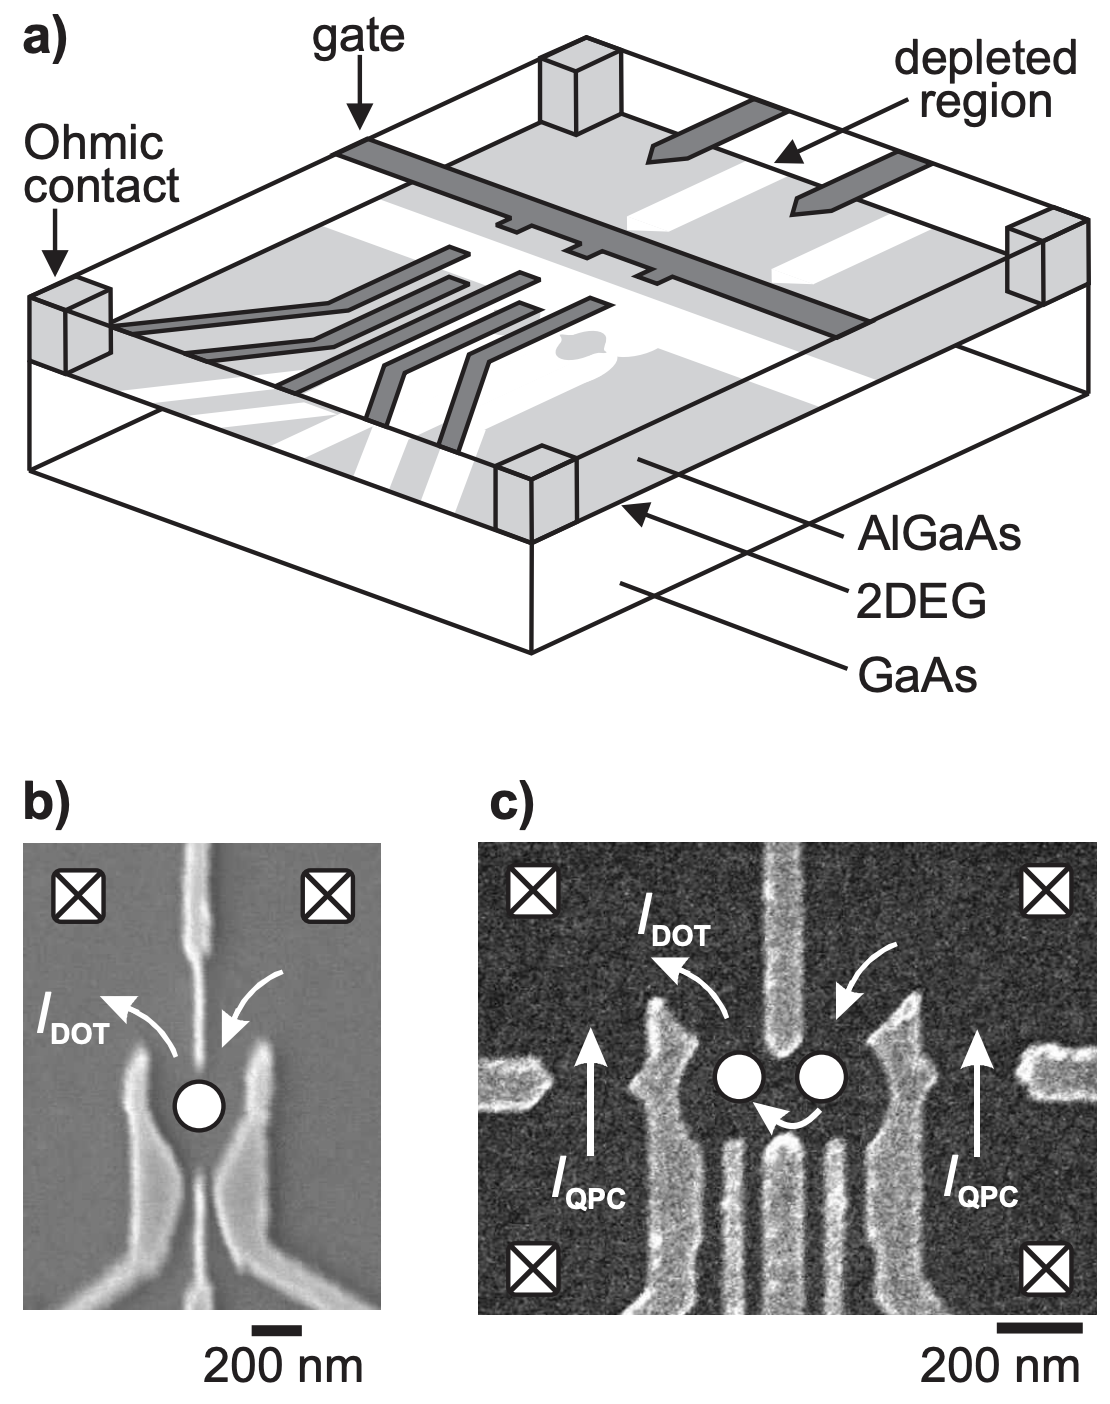
\includegraphics[width=0.5\linewidth]{images/Hanson-1.png}
    \caption{Изображение квантовой точки, наведенной при помощи латеральных затворов. \cite{ref:Hanson2007}}
    \label{fig:lateral_schema}
\end{figure}

Из вышеприведенных оценок можно сделать вывод, что подобные устройства могут работать только при очень низких температурах (порядка нескольких кельвинов), при этом напряжения на затворах могут быть реализованы без особых ухищрений.

\subsection{Квантовый бит}

Рассмотрим сферу Блоха — модельное представление, используемое для описания операций с одиночным кубитом.
Кубит является простейшей квантово-механической системой и обобщает классический бит. Будучи двухуровневой системой, кубит может находиться в одном из базисных состояний, обозначаемых \(\ket{0}\) и \(\ket{1}\), что соответствует классическим значениям 0 и 1. Однако ключевое отличие кубита от классического бита заключается в возможности находиться в суперпозиции этих состояний:

\begin{equation}
\ket{\psi} = a\ket{0} + b\ket{1},
\label{eq:qubit_superposition}
\end{equation}

где \(a\) и \(b\) — комплексные числа, называемые амплитудами вероятности. Таким образом, состояние кубита описывается вектором в двумерном комплексном пространстве \(\mathbb{C}^2\), а выражение \eqref{eq:qubit_superposition} можно интерпретировать как интерференцию двух возможностей. Геометрически такое состояние изображается точкой на сфере Блоха (рис.~\ref{fig:bloch_sphere}), причём связь между коэффициентами и углами \((\theta, \varphi)\) задаётся формулой
\[
\ket{\psi} = \cos\frac{\theta}{2}\ket{0} + e^{i\varphi}\sin\frac{\theta}{2}\ket{1},
\]
где \(0 \le \theta \le \pi\), \(0 \le \varphi < 2\pi\).

\begin{figure}[h]
\centering
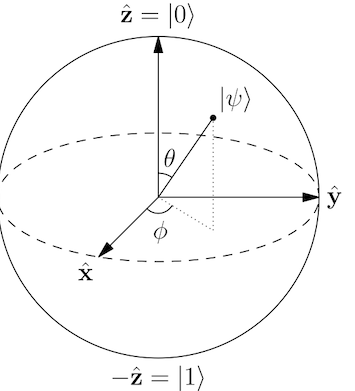
\includegraphics[width=0.8\textwidth]{images/Bloch_Sphere.png}
\caption{Сфера Блоха}
\label{fig:bloch_sphere}
\end{figure}

\subsubsection{Несколько кубитов}

Состояние двух кубитов, каждый из которых находится в произвольном состоянии суперпозиции
$\ket{\psi}_1 = a_1 \ket{0} + b_1 \ket{1}$ и $\ket{\psi}_2 = a_2
\ket{0} + b_2 \ket{1}$, записывается как
%
\begin{equation}
\ket{\psi} = \ket{\psi}_1 \otimes \ket{\psi}_2
= (a_1 \ket{0} + b_1 \ket{1}) \otimes (a_2 \ket{0} + b_2 \ket{1}) \,,
\label{eq:product_qubits}
\end{equation}
%
где $\otimes$ — это символ {\em тензорного произведения}.
Выражение можно записать как
\begin{equation}
\ket{\psi} = 
c_{00} \ket{00} + c_{01} \ket{01} + 
c_{10} \ket{10} + c_{11} \ket{11} \,.
\end{equation}
\noindent Или, что эквивалентно, если мы представим состояния в десятичной записи вместо двоичной:
\begin{equation}
\ket{\psi} = 
c_{0} \ket{0} + c_{1} \ket{1} + c_{2} \ket{2} + c_{3} \ket{3} \,.
\label{eq:psi_c_i}
\end{equation}
%
Аналогичным образом, регистр из $n$ кубитов может находиться в произвольной
суперпозиции $2^n$ состояний:
\begin{equation}
\ket{\psi} = \sum_{k=0}^{2^n-1} c_k \ket{k} \,,
\label{eq:general_superposition}
\end{equation}
где единственным ограничением для комплексных амплитуд $c_k$ является то,
что они должны удовлетворять условию нормировки
\begin{equation}
\sum_k |c_k|^2 = 1 \,.
\label{eq:normalization}
\end{equation}
Как и для однокубитных состояний, общая фаза не имеет
значения.

\noindent Это кардинально отличается от классических систем. Например, 
положение $n$ точек на сфере, показанной на рис.~\ref{fig:bloch_sphere}, 
описывается всего $n$, а не $2^n$ комплексными числами. Фактически, положение
любых $n$ классических частиц всегда можно описать количеством действительных или 
комплексных чисел, зависящим от $n$ линейно. Поэтому невозможно описать геометрически состояние двух и более кубитов.

\subsubsection{Запутанность}

Поскольку число степеней свободы $n$ квантовых систем растет экспоненциально быстрее,
чем у $n$ классических систем, несомненно, должны существовать квантовые состояния,
которые не имеют классических аналогов.
Состояние, описываемое уравнением~\ref{eq:product_qubits},
является «классическим»: это совместное состояние двух кубитов может быть полностью
описано через параметризацию отдельных кубитов (для чего требуется одно комплексное 
либо два действительных числа на каждый кубит). Мы говорим, что 
состояние из уравнения~\ref{eq:product_qubits} является {\em сепарабельным} (разделимым).

В противоположность этому, невозможно найти два однокубитных состояния
$\ket{\psi}_1 = a_1 \ket{0} + b_1 \ket{1}$ и $\ket{\psi}_2 = a_2
\ket{0} + b_2 \ket{1}$ такие, чтобы их тензорное произведение давало состояние
\begin{equation}
\frac{\ket{00}+\ket{11}}{\sqrt{2}} \,.
\label{eq:epr}
\end{equation}
Другими словами, это состояние нельзя записать как произведение двух
однокубитных состояний. Такое состояние мы называем {\em несепарабельным} 
или {\em запутанным}. Приведем еще два примера: состояние $\frac{1}{2}
(\ket{00} - \ket{01} + \ket{10} - \ket{11})$ можно записать как
$\frac{1}{2} (\ket{0} + \ket{1})(\ket{0}-\ket{1})$, и, следовательно, оно 
является сепарабельным; в то время как состояние $\frac{1}{2} (\ket{00} + \ket{01} +
\ket{10} - \ket{11})$ нельзя разложить на два однокубитных состояния, поэтому
оно является запутанным. Запутанное состояние - ключевое преимущество квантовой системы над классической.

\subsection{Использование квантовых систем для вычислений}
Чтобы выолнять опреации с данными, которые в квантовом компьютере закодированы в кубитах необходимо определть, как и в классическом компьютере базовые вентили. 

Однокубитные вентили могут быть записаны в виде матриц Паули:
\begin{equation}
\sigma_x \equiv \begin{pmatrix} 0 & 1 \\ 1 & 0 \end{pmatrix}, \quad
\sigma_y \equiv \begin{pmatrix} 0 & -i \\ i & 0 \end{pmatrix}, \quad
\sigma_z \equiv \begin{pmatrix} 1 & 0 \\ 0 & -1 \end{pmatrix},
\end{equation}
которые удовлетворяю условиям
\begin{equation}
\sigma_x \sigma_y = i \sigma_z \,, \quad
\sigma_x \sigma_z = - i \sigma_y \,, \quad
\sigma_y \sigma_z = i \sigma_x \,, \quad
\label{eq:pauli_rel1}
\end{equation}
\begin{equation}
\sigma_x^2 = \sigma_y^2 =  \sigma_z^2 = \sigma_I \,,
\label{eq:pauli_rel2}
\end{equation}
где 
\begin{equation}
\sigma_I \equiv \begin{bmatrix} 1 & 0 \\ 0 & 1 \end{bmatrix}.
\end{equation}

Вентиль $\sigma_x$ очень похож на классический вентиль NOT: он преобразует |0〉 в |1〉, а |1〉 в |0〉. Эта операция эквивалентна повороту вектора на сфере Блоха вокруг оси x на $\pi$  радиан (или 180°).

Вентиль $\sigma_y$ ожидаемо соответствует повороту вектора вокруг оси y на $\pi$ радиан. В результате такой операции вектор |0〉 превращается в i|1〉, а |1〉 — в -i|0〉.

Вентиль $\sigma_z$ представляет собой особый случай вентиля фазового сдвига. Вектор |0〉 он оставляет без изменений, а |1〉 преобразует в -|1〉.

Также есть вентиль именнуемы вентилем Адамара, он представляет так же особую важность так как может преобразовывать в суперпозицию состояний.
%
\begin{equation}
H = \frac{1}{\sqrt{2}} \begin{bmatrix} 1 & 1 \\ 1 & -1 \end{bmatrix}.
\end{equation}
%
\begin{equation}
\ket{0} \stackrel{\textstyle H}{\longleftrightarrow} \frac{\ket{0}+\ket{1}}{\sqrt{2}} 
\quad \mbox{and} \quad
\ket{1} \stackrel{\textstyle H}{\longleftrightarrow} \frac{\ket{0}-\ket{1}}{\sqrt{2}} \,.
\label{eq:Had_effect}
\end{equation}
%
Существуют также и двух кубитные вентили.
\begin{equation}
    U_{\mbox{\sc cnot}} = \begin{bmatrix} 1 & 0 & 0 & 0 \\ 
                                            0 & 1 & 0 & 0 \\ 
                                            0 & 0 & 0 & 1 \\ 
                                            0 & 0 & 1 & 0 \end{bmatrix} \quad
\end{equation}
\begin{equation}
U_{\mbox{\sc swap}} = \begin{bmatrix} 1 & 0 & 0 & 0 \\ 
                                       0 & 0 & 1 & 0 \\ 
                                       0 & 1 & 0 & 0 \\ 
                                       0 & 0 & 0 & 1 \end{bmatrix},
\end{equation}

CNOT — это обратимый логический вентиль, реализующий операцию, сходную с классическим XOR. Имеет 2 входа и 2 выхода. Первый вход — управляющий сигнал, второй вход — бит, который будет инвертирован в случае, если на управляющем входе подана единица.

SWAP - это, соотвественно, вентиль, который меняет между собой местами два своих входа.
\subsubsection{Квантовый параллелизм}
Любое вычисление можно рассматривать как последовательную цепочку (конкатенацию) множества логических вентилей. Каждый логический вентиль генерирует выходное значение, которое является функцией от его входного сигнала. Теперь рассмотрим классический и обратимый логический вентиль, который реализует функцию $f$ с одним входным битом $x$ и одним выходным битом $y=f(x)$. Если $x=0$, вентиль выдаст $f(0)$, а если $x=1$, вентиль выдаст $f(1)$. Теперь представьте, что мы можем реализовать аналогичный квантовый логический вентиль, который преобразует кубит как $\ket{x} \mapsto
\ket{f(x)}$. В силу линейности квантовой механики, этот же квантовый вентиль преобразует кубит, находящийся в состоянии суперпозиции, следующим образом:
%
\begin{equation}
a \ket{0} + b \ket{1} \quad \stackrel{f}{\mapsto} \quad
 a \ket{f(0)} + b \ket{f(1)} \,.
\label{eq:1qubit_out}
\end{equation}
%
В некотором смысле, функция $f$ была вычислена для обоих её входных значений ($0$ и $1$) за один шаг. Далее рассмотрим другой логический вентиль, который реализует функцию $f$ с двумя входными и двумя выходными битами. Если мы приготовим двухкубитную систему в состоянии
%
\begin{equation}
\ket{\psi} = a \ket{00} + b \ket{01} + c \ket{10} + d \ket{11} \,,
\label{eq:2qubits_in}
\end{equation}
%
вычисление функции $f$ преобразует это состояние в
%
\begin{equation}
a \ket{f(00)} + b \ket{f(01)} + c \ket{f(10)} + d \ket{f(11)} \,,
\label{eq:2qubits_out}
\end{equation}
%
и таким образом, $f$ была вычислена для четырёх входных значений параллельно. В общем случае, функция от $n$ битов, реализованная на квантовом компьютере, может быть вычислена для всех $2^n$ возможных входных значений одновременно:
%
\begin{equation}
\sum_{x=0}^{2^n-1} c_x \ket{x} \quad \stackrel{f}{\mapsto} \quad
\sum_{x=0}^{2^n-1} c_x \ket{f(x)} \,,
\label{eq:nqubits_out}
\end{equation}
%
где $x$ — это целое число, закодированное строкой из $n$ битов. Таким образом, в то время как для классических компьютеров число параллельных вычислений функции растет в лучшем случае линейно в зависимости от их размера,
{\em количество параллельных вычислений функции экспоненциально возрастает с увеличением размера квантового компьютера (числа кубитов).}

\noindent Эта концепция была впервые предложена 
Дэвидом Дойчем (David Deutsch) в 1985 году и получила название {\em квантового
параллелизма} \cite{Deutsch85a}.

\subsection{Вычисления на основе квантовых точек}

В работе \cite{ref:Loss1998} Дениэль Лосс и Девид ДеВенченцо описали сценарий, с помощью которого можно реализовать квантовые вычисления в системе связанных квантовых точек. В их модели кубит реализован в виде спина избыточного электрона на квантовой точке с одним электроном. Работа с кубитами основана на чисто электрическом регулировании туннельного барьера между соседними квантовыми точками.

Взаимодействие между двумя соседними спинами $\mathbf{S}_1$ и $\mathbf{S}_2$, согласно модели Хаббарда описывается гамильтонианом Гейзенберга:
\begin{equation}\label{eq1}
    H(t) = J(t) \cdot \mathbf{S}_1 \cdot \mathbf{S}_2,
\end{equation}
где $J(t)$ — энергия обменного взаимодействия. Включая это взаимодействие на определенное время $\tau$, можно реализовать операцию $\sqrt{\text{SWAP}}$, которая является универсальным двухкубитным вентилем.

Отмечается, что
\begin{equation}
    J(t) \approx \frac{4t_c(t)^2}{U}.
\end{equation}

— зависящая от времени константа обмена, возникающая при включении и выключении матричного элемента туннелирования $t_c(t)$. $U$ — энергия зарядки одной квантовой точки.


Уравнение \ref{eq1} хорошо описывает систему квантовых точек при соблюдении нескольких условий.
\begin{enumerate}
    \item  Можно не учитывать более высоколежащие одночастичные состояния квантовых точек. Для этого необходимо, чтобы $\delta E >> kT$, где $\delta E$ — расстояние между уровнями, а $T$ — температура.
    \item Время $\tau_s$, в течение которого потенциал затвора остается низким, должно быть больше, чем $\frac{\hbar}{\delta E}$, чтобы предотвратить переходы на более высокие орбитальные уровни
    \item $U >> t_c(t)$ это необходимо, чтобы приближение гейзенберга оставалось достаточно точным
    \item Время декогеренции $\Gamma^{-1}$ должно быть намного больше времени переключения $\tau_s$,
\end{enumerate}

Если время декогеренции $\Gamma^{-1}$ достаточно велико, то может быть достигнут идеал квантовых вычислений, при котором действие импульсного гамильтониана сводится к применению унитарного оператора эволюции 
\[U_s(t) = T \exp\left\{-i \int_0^t H_s(t') dt'\right\}\]
к начальному состоянию двух спинов: $|\Psi(t)\rangle = U_s |\Psi(0)\rangle$. 
Импульсная гейзенберговская связь приводит к специальной форме оператора $U_s$: 
при определённой длительности $\tau_s$ спин-спинового взаимодействия, такой что 
$\int J(t) dt = J_0 \tau_s = \pi$ (по модулю $2\pi$), 
оператор $U_s(J_0\tau_s = \pi) = U_{\text{sw}}$ становится оператором ``обмена'' (swap): 
если $|ij\rangle$ обозначает базисные состояния двух спинов в $S_z$-базисе, где $i,j = 0,1$, 
то $U_{\text{sw}}|ij\rangle = |ji\rangle$. 
Поскольку этот оператор сохраняет полный момент импульса системы, 
одного только $U_{\text{sw}}$ недостаточно для выполнения полезных квантовых вычислений. 
Однако если взаимодействие включается на половину этой длительности, 
то получаемый ``квадратный корень из обмена'' $U_{\text{sw}}^{1/2}$ оказывается очень полезным в качестве базового квантового логического элемента. 
Например, квантовый элемент CNOT может быть реализован с помощью простой последовательности операций:
\begin{equation}
U_{\text{CNOT}} =
%e^{-i{3\pi\over 4}}
e^{i \frac{\pi}{2} S_1^z} e^{-i \frac{\pi}{2} S_2^z}
U_{\text{sw}}^{\frac{1}{2}} e^{i\pi S_1^z} U_{\text{sw}}^{\frac{1}{2}},
\label{CNOT}
\end{equation}
где $e^{i\pi S_1^z}$ и аналогичные члены — одночастичные операции, 
которые могут быть реализованы, например, с помощью локальных магнитных полей. 
Совместно с одночастичными операциями элемент CNOT позволяет реализовать любое квантовое вычисление.

\subsection{Использование квантвых точек}
В настоящее время существует ряд работ (\cite{tadokoro2021}, \cite{shutling}), в которых осуществлен теоретическиский расчет различных аспектов квантовых вычислительных устройств на полупроводниковых квантовых точках.

Так например, cтатья \cite{tadokoro2021} посвящена разработке практических дизайнов двумерных массивов квантовых точек в кремнии для масштабируемых квантовых процессоров. Основная цель — обеспечить связность каждого кубита с четырьмя ближайшими соседями при сохранении индивидуальной адресуемости. Рассматриваются два масштаба: компактный массив $3\times 3$ (9 точек) и перспективный дизайн для интеграции более тысячи кубитов.

\subsubsection{Дизайн массива $3\times 3$ квантовых точек}

Основной предлагаемый дизайн — массив из девяти квантовых точек, сформированных в гетероструктуре Si/SiGe. 
\begin{figure}
    \centering
    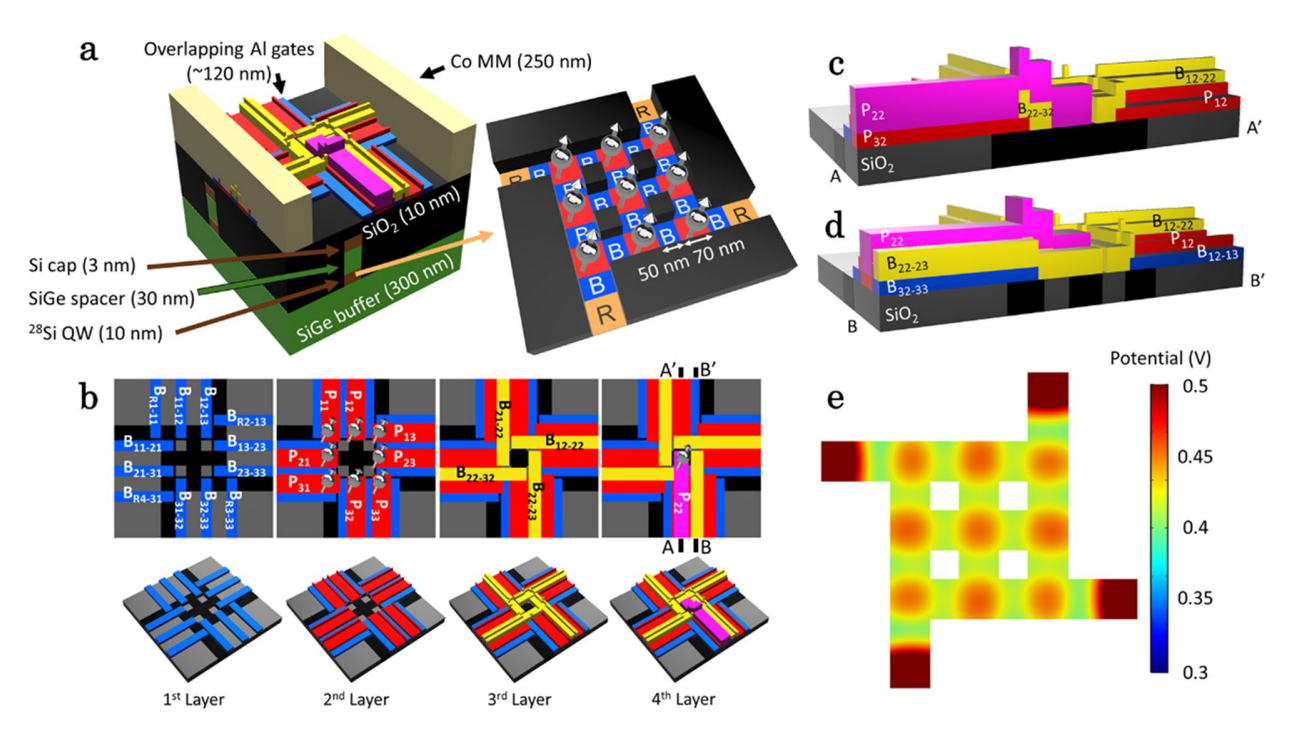
\includegraphics[width=1.0\linewidth]{images/design.png}
    \caption{Пример дизайна структуры кубитов 3x3 из работы \cite{tadokoro2021}}
    \label{fig:placeholder}
\end{figure}

Геометрические параметры:
\begin{itemize}
    \item Области квантовых точек: квадраты размером \textbf{$70\times 70$ нм} (обозначены красным).
    \item Разделительные барьерные затворы: ширина \textbf{50 нм} (темно-синие области). Они контролируют обменное взаимодействие между соседними точками.
    \item Резервуары (источники электронов): оранжевые области.
\end{itemize}

\begin{table}[htbp]
\centering
\caption{Характеристики слоев перекрывающихся затворов}
\label{tab:layers}
\small % чуть уменьшить шрифт
\begin{tabularx}{\textwidth}{@{}>{\hsize=0.8\hsize}X 
                            >{\hsize=1.2\hsize}X 
                            >{\hsize=0.6\hsize}X 
                            >{\hsize=0.6\hsize}X 
                            >{\hsize=0.8\hsize}X@{}}
\toprule
Номер слоя & Назначение & Цвет на схеме & Ширина (нм) & Высота (нм) \\ \midrule
1 & Барьерные затворы ($B_{11-12}$ и др.) & Синий & 50 & 15 \\
2 & Плунжерные затворы ($P_{11}$, $P_{12}$...) & Красный & 90 & 25 \\
3 & Барьерные затворы ($B_{11-12}$ и др.) & Желтый & 60 & 40 \\
4 & Плунжерный затвор ($P_{22}$) & Пурпурный & 70 & 60 \\ \bottomrule
\end{tabularx}
\end{table}

\subsubsection{Электростатическое моделирование}
С помощью COMSOL Multiphysics авторы подтвердили формирование девяти изолированных квантовых ям в кремниевой квантовой яме при комнатной температуре. Использованные напряжения:
\begin{itemize}
    \item На плунжерных затворах: \textbf{0.6 В}.
    \item На барьерных затворах между точками: \textbf{0.4 В}.
    \item На барьерных затворах между точкой и резервуаром: \textbf{0.3 В}.
\end{itemize}

\subsubsection{Управление спинами}
Для индивидуального управления спинами (однокубитные и двухкубитные операции) используется техника EDSR (Electric Dipole Spin Resonance) с помощью микромагнитов (MM).

\subsubsection{Обсуждение}
В итоге авторы показывают возможность обеспечения адресации кубитов в двумерном массиве из \(3\times 3\) квантовых точек, который может более эффективно выполнять квантовые схемы по сравнению с одномерным массивом. Этот метод в основном основан на экспериментально реализованных структурах ММ и КТ с возможностью создания квантовых устройств.

Однако в данной работе отсутствует расчет волновых функций и энергетического спектра квантовых точек для предложенной системы. Авторы ограничились классическим электростатическим моделированием потенциала в квантовой яме, не переходя к квантово-механическому анализу одночастичных и многочастичных состояний. Это не позволяет оценить ряд ключевых параметров:
\begin{itemize}
    \item \textbf{Орбитальное расщепление} \(E_{\text{orb}}\) — энергетический зазор между основным и первым возбужденным состоянием в каждой точке, определяющий чувствительность к зарядовому шуму и времена жизни кубита.

    \item \textbf{Обменное расщепление} \(J\) между соседними точками — ключевой параметр для реализации двухкубитных вентилей. Его зависимость от напряжения на барьерных затворах и однородность по массиву остались неисследованными.
\end{itemize}
Таким образом, предложенный дизайн требует дальнейшей теоретической проверки с использованием методов, учитывающих квантовую природу электронов в наноструктурах. Расчет энергетического спектра наведенных квантовых точек, включая орбитальные и долинные состояния, а также оценка влияния беспорядка на однородность массива, являются необходимым следующим шагом для подтверждения реализуемости масштабируемого квантового процессора на основе данной архитектуры. Именно это направление и составляет цель настоящей дипломной работы, позволяя дополнить и углубить результаты, полученные в статье \cite{tadokoro2021}.

Рассмотрим также статью \cite{shutling}. В ней рассматривается такой аспект квантовых схем, как передача информации между квантовыми регистрами.

В данной статье авторы экспериментально исследуют метод механического перемещения электрона с сохранением его спинового состояния через линейный массив квантовых точек.

Авторы предлагают методологию перемещения кубита, которая называется "Bucket-brigade". Суть ее заключается в том, что электрон транспортируется через массив квантовых точек путем послеовательнй регулировки потенциалов электродов, которыми они наводятся. Авторы демонстрируют в работе перемещение электрона вперед и назада через массив на расстояние до 1000 скачков, что эквивалентно 80 мкм. В конце проверяется сохраняется ли спиновая поляризация.

Устройство имеет следующий вид. Массив квантовых точек (Рис.~\ref{fig:shuttle}) изготовлен на
нелегированной гетероструктуре Si/SiGe, при этом квантовая яма
расположена на глубине 30 нм ниже поверхности.

Устройство содержит три слоя затворных электродов,
используемых, соответственно, в качестве экранирующих затворов, плунжерных и
накопительных затворов, а также барьерных затворов, изолированных между ними диэлектрическими слоями. Устройство может вмещать линейный
массив до пяти квантовых точек с шагом 80 нм.
Точки формируются путем приложения напряжения к металлическим
затворным электродам, где плунжерные затворы позволяют регулировать
электрохимические потенциалы квантовых точек,
а барьерные затворы контролируют туннельные связи между
квантовыми точками. Все измерения проводятся в криостате с разбавлением при
базовой температуре ниже 20 мК.

\begin{figure}
    \centering
    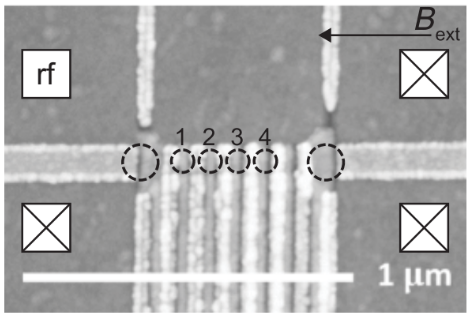
\includegraphics[width=0.5\linewidth]{images/shuttle.png}
    \caption{Изображение устройства, полученное с помощью сканирующего электронного микроскопаю. Квантовые точки обозначены маленькими кружками. Левый
датчик подключен к схеме считывания ВЧ-сигнала через один из омических резервуаров, обозначенных квадратами. \cite{shutling}}
    \label{fig:shuttle}
\end{figure}

\subsubsection{Обсуждение}
Эксперимент был выстроен в соответствии со строгой
методологической последовательностью:
\begin{enumerate}
    \item \textbf{Инициализация состояния.} Внешним магнитным полем ($B_0 = 1.3$~Тл) в системе создавалось зеемановское расщепление уровней энергии спина. Путем точной настройки напряжения на затворе над первой квантовой точкой (КТ1) в нее загружался одиночный электрон из электронного резервуара. Электрон попадал в систему со случайной поляризацией: спин <<вверх>> ($|\!\uparrow\rangle$) или <<вниз>> ($|\!\downarrow\rangle$) с вероятностью 50\%.
    
    \item \textbf{Процесс пространственного перемещения (shuttling).} Путем адиабатического изменения электростатического потенциала на соседних затворах электрон поочередно преодолевал барьеры, перемещаясь от КТ1 до КТ3 (или КТ4) и обратно. Ключевая идея данного этапа заключалась в независимом варьировании двух параметров: общего времени нахождения электрона в массиве ($t_{\text{total}}$) и количества совершенных им межузельных перескоков ($N$).
    
    \item \textbf{Считывание квантового состояния.} По завершении заданного числа циклов электрон возвращался в исходную КТ1. Для определения его спинового состояния применялся метод спин-зависимого туннелирования (spin-to-charge conversion). Электрохимический потенциал точки настраивался таким образом, что уровень Ферми резервуара оказывался строго между двумя зеемановскими подуровнями электрона. В результате электрон со спином $|\!\uparrow\rangle$ туннелировал в резервуар, что фиксировалось высокочувствительным зарядовым сенсором как кратковременный всплеск тока. Электрон со базисном состоянии $|\!\downarrow\rangle$ преодолеть барьер не мог, и сигнал на сенсоре отсутствовал.
    
    \item \textbf{Статистическое доказательство сохранения спина.} Повторив описанный процесс от 500 до 1000 раз для каждого набора параметров, авторы проанализировали статистику. Главный результат заключался в следующем: вероятность обнаружения спина $|\!\uparrow\rangle$ оказалась абсолютно независимой от количества физических перескоков $N$. Падение поляризации зависело только от общего времени $t_{\text{total}}$, проведенного электроном в массиве. 
\end{enumerate}

Из этого был сделан важнейший физический вывод:  физический акт преодоления потенциального барьера практически не вносит вклад в разрушение спинового состояния электрона.

В данной работе авторами успешно демонстрируется работоспособность подобной архитектуры спинового шатла. Но при этом ими же отмечается тот факт, что необходимо сконцентрировать услилия на увеличении скорости тунелирования между квантовыми точками. Такое проще реализовать имея перед собой готовую рассчитанную модель подобного устройства, что и делается в данной работе.

\subsection{Наведённые квантовые точки в кремниевых наноструктурах}
\label{ch:si_qd}

Наведённые квантовые точки в кремниевых наноструктурах являются одним из
наиболее перспективных физических воплощений твердотельных кубитов. Данная работа концентрируется 
именно на таком варианте реализации, квантовых точек. В связи с этим, расмотрим на примере 
нескольких современных работ особенности квантовых точек в кремннии.

%----------------------------------------------------------------
\subsubsection{Особенности квантовых точек на основе крмения}
\label{sec:features}
%---------------------------------------------------------------- 

Основываясь на работе \cite{Chatterjee2021} можно сказать, что хоть гетероструктуры 
на основе $GaAs$ сыграли ключевую роль в разработке квантовых точек, 
то сейчас основное внимание исследователей сосредоточено на наноструктурах на 
основе кремния из-за их потенциала в области квантовых вычислений на основе спина. 

Это связанно с тем. что изотопно очищенный кремний, обогащенный $Si^{28}$, 
не обладающим ядерным спином, обеспечивает длительное время жизни спина. Кроме того, 
кремний — привлекательный материал для крупномасштабной интеграции. Однако из-за большей 
эффективной массы кремния характерный размер квантовых точек должен быть меньше, 
чем в арсениде галлия, то есть составлять менее \textbf{20 нм}, что усложняет процесс 
нанолитографии.

\textbf{Зарядовый кубит в кремнии}

На основе наведенных квантовых точек в кремнии можно создать зарядовый кубит, если 
взять две таких стоящих рядом. В таком случае расположение электрона в обдной из них
будет оначать соответсвенно состояния $\ket{0}$ или $\ket{1}$. Но при этом у кремния есть особенность,
которая выделяет его. Многодолинная природа зоны проводимости кремния приводит к тому, что при 
ограничении степеней свободы происходит так называемое долинное расщепление, то есть в кантовой точке
появляются два различных состояния, которые можно интерпретировать как $\ket{0}$ и $\ket{1}$.


\textbf{Спиновый кубит в кремнии}

Еще одна особенность кремния, которая выделяет его на фоне того же $GaAs$ заключается в том, что только
малая часть атомов в кремнии яввляется изотопами. Из за этого время когерентности кубита значительно вырастает
и начинает сильно превышать время выполнение операций. Опираясь на работу \cite{Chatterjee2021}, можно
привести следующие значения времени когерентности: $t \thicksim 10$ мкс, а иногда
даже превышает 120 мкс.
%----------------------------------------------------------------
\subsubsection{Платформы и геометрия затворных систем}
\label{sec:geometry}
%----------------------------------------------------------------

Квантовые точки на основе кремния имеют также преимущество в том, что могут быть
изготовлены при помощи промышленных технологий. Это было показанно в работе 
\cite{Zwerver2022}. Авторы предоставили устройство, которое состояло из двух кремниевых 
нанопроводов шириной \textbf{от 20 до 70 нм}, но одном располагались наведенные квантовые точки, 
а на другом - зарядовыве сенсоры.
Расстояние между ними составляло примерно \textbf{150 нм}.
Сверху они были наркыты затворами шириной около \textbf{50 нм} (Рис. \ref{fig:Zwerver}).

В данной работе наведенные квантовые точки играли роль спиновых кубитов, считвыание значений которых
производилось при помощи зарядовых сенсоров. Вращение же спина осужествлялось при помощи тока, который
создавал вокруг себя переменное магнитное поле, вызывающее электронный спиновый резонанс между уровнями,
созданными при помощи зеемановского расщепления.

По итогу авторы измерили время спиновой релаксации ($\thicksim 1 c$) и время когерентности 
($\thicksim 24$ мкс). При этом точность однокубитных операций составляет $99\%$. 
Таким образом авторы показали что можно создавать кубиты на основе квантовых точек в кремнии, что
делает их по настоящему перспективными в будущем развитии технологий.

\begin{figure}
    \centering
    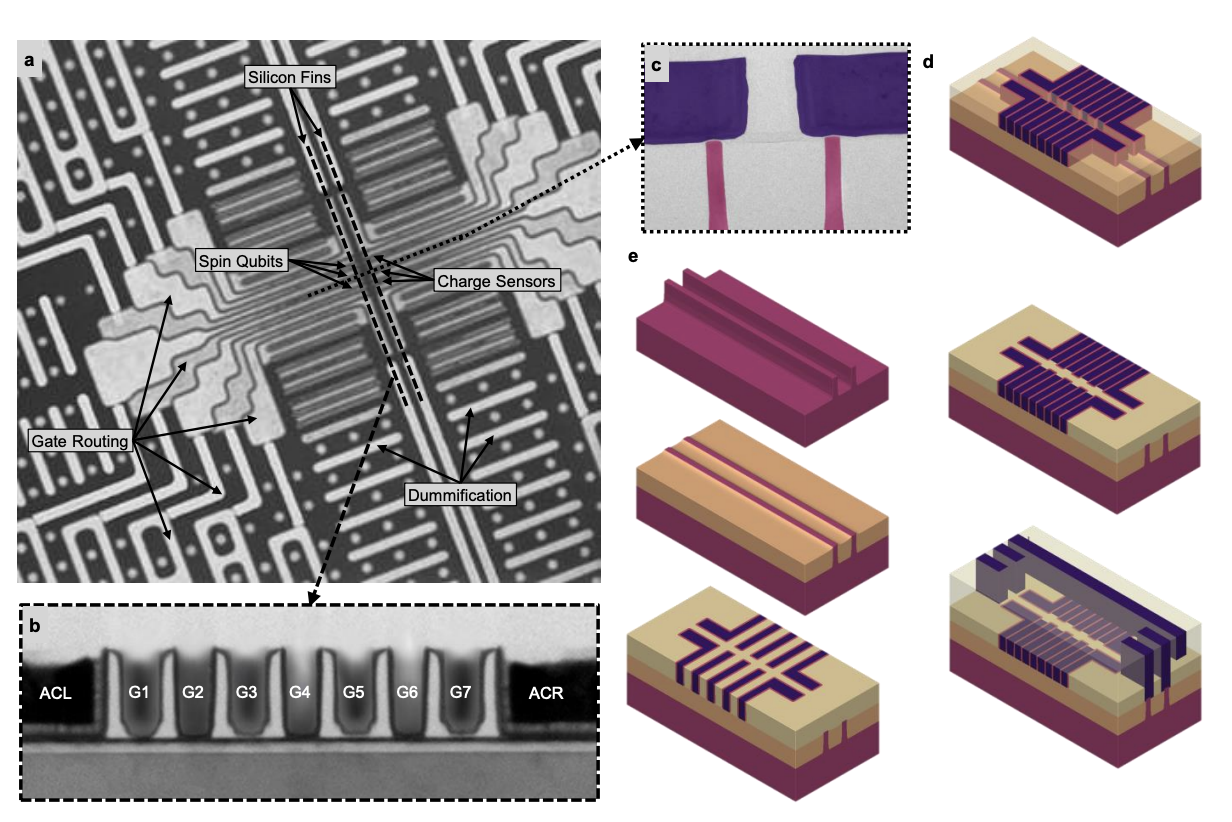
\includegraphics[width=1.0\linewidth]{images/Zwerver.png}
    \caption{\textbf{(a)} Изображение устройства, полученное на электронный микроскоп. 
    \textbf{(b)} Изображение вдоль кремниевого нанопровода, показывающее 7 затворов, наводящих массив квантовых точек: G1--G7, и два затвора стока и истока: ACR и ACL соответственно. 
    \textbf{(c)} Изображение нанопроводов и затворов сверху. 
    \textbf{(d)} Схема активной области устройства. 
    \textbf{(e)} Схема технологических этапов, используемых для изготовления устройств. \cite{Zwerver2022}}
    \label{fig:Zwerver}
\end{figure}

\chapter{Актульность и цели работы}
\textbf{\underline{Актуальность работы}}

В элементах полупроводниковых квантовых компьютеров с большим числом кубитов необходимо большое число туннельных и управляющих электродов, а также большое количество островков. Причём, изменение взаимного расположения этих элементов координально меняет транспортные, зарядовые, спиновые и временные характеристики устройства, а также влияет на качество его работы. Так как изготовление реальных образцов с определенным расположением элементов является очень долгой и дорогостоящей процедурой, необходимо производить предворительный расчёт интересующих транспортных характеристик реализуемого устройства. Численное моделирование позволит быстро менять расположение элементов, добавлять новые составляющие устройства, а также подбирать их оптимальную форму и размер, благодаря чему в последствии можно будет изготовить устройство с максимальным временем квантовой когерентности и квантовой достоверности для выполнния квантовых операций. 

Кремниевые спиновые кубиты обладают длительным временем когерентности и технологически совместимы с индустриальными литографическими процессами. Однако плотное двумерное размещение кубитов в матрице затруднено из-за так называемой проблемы расслоения управляющих линий. Для её решения предложены различные схемы средне-дальней передачи информации, включая перенос одиночных электронов на расстояния порядка 10 мкм. Для более быстрого и удобного анализа подобных устройств необходима компьютерная модель.

В связи с этим, данная работа является десйствительно актуалной.


\textbf{\underline{Цели работы}}


Основной целью данной дипломной работы является разработка численной модели, позволяющей с нуля рассчитывать энергетический спектр и волновые функции наведенных квантовых точек в массивах на основе Si/SiGe гетероструктур.

Для достижения поставленной цели необходимо решить следующие задачи:
\begin{enumerate}
    \item \textbf{Построение электростатической модели} сложной затворной структуры.
    \item Решение уравнения Лапласа для определения потенциала и напряженности поля для заданной стнркутуры при определенных граничгых условиях.
    \item \textbf{Расчет энергетического спектра} в каждой квантовой точке путем решения уравнения Шрёдингера для электрона в полученном потенциале. Определение основного и возбужденных орбитальных состояний.
    \item \textbf{Анализ рассчетов} получившихся значений параметров для предложенных дизайнов структур.
\end{enumerate}

Ожидаемые результаты работы позволят не только подтвердить корректность разработанной модели, но и дать количественные рекомендации для изготовления для реализации масштабируемого квантового процессора на спинах электронов в кремнии. Тем самым будет внесен вклад в развитие методов моделирования и оптимизации архитектур квантовых устройств.

\chapter{Техничекская реализация}
\section{Создание модели}
Базовым элементом модели, на которой будет производится рассчет является параллепипед, на его основе строятся такие элементы как:
\begin{enumerate}
    \item Нанопровод
    \item Затворный электрод
    \item Оксиды покрывающие элементы
\end{enumerate}

Примерная структура представлена на рисунке ниже (Рис. \ref{fig:model})

Структура задается программно, что позволяет гибко манипулировать параметрами модели. Так нпример, есть возиожность регулировать размеры любого элемента, манипулировать позиционированием затворов, степенью огибания завтором наномостика. Так же есть возможность задать любое количество затворов на наномостике, каждый из которых имеет гибкую настройку описанную выше.

Ниже приведены примеры моделей,которые можно сделать при помощи программы.
(Рис. \ref{fig:model}, Рис. \ref{fig:model_3electrodes}, 
Рис. \ref{fig:model_many_electrodes})

\begin{figure}[]
    \centering
    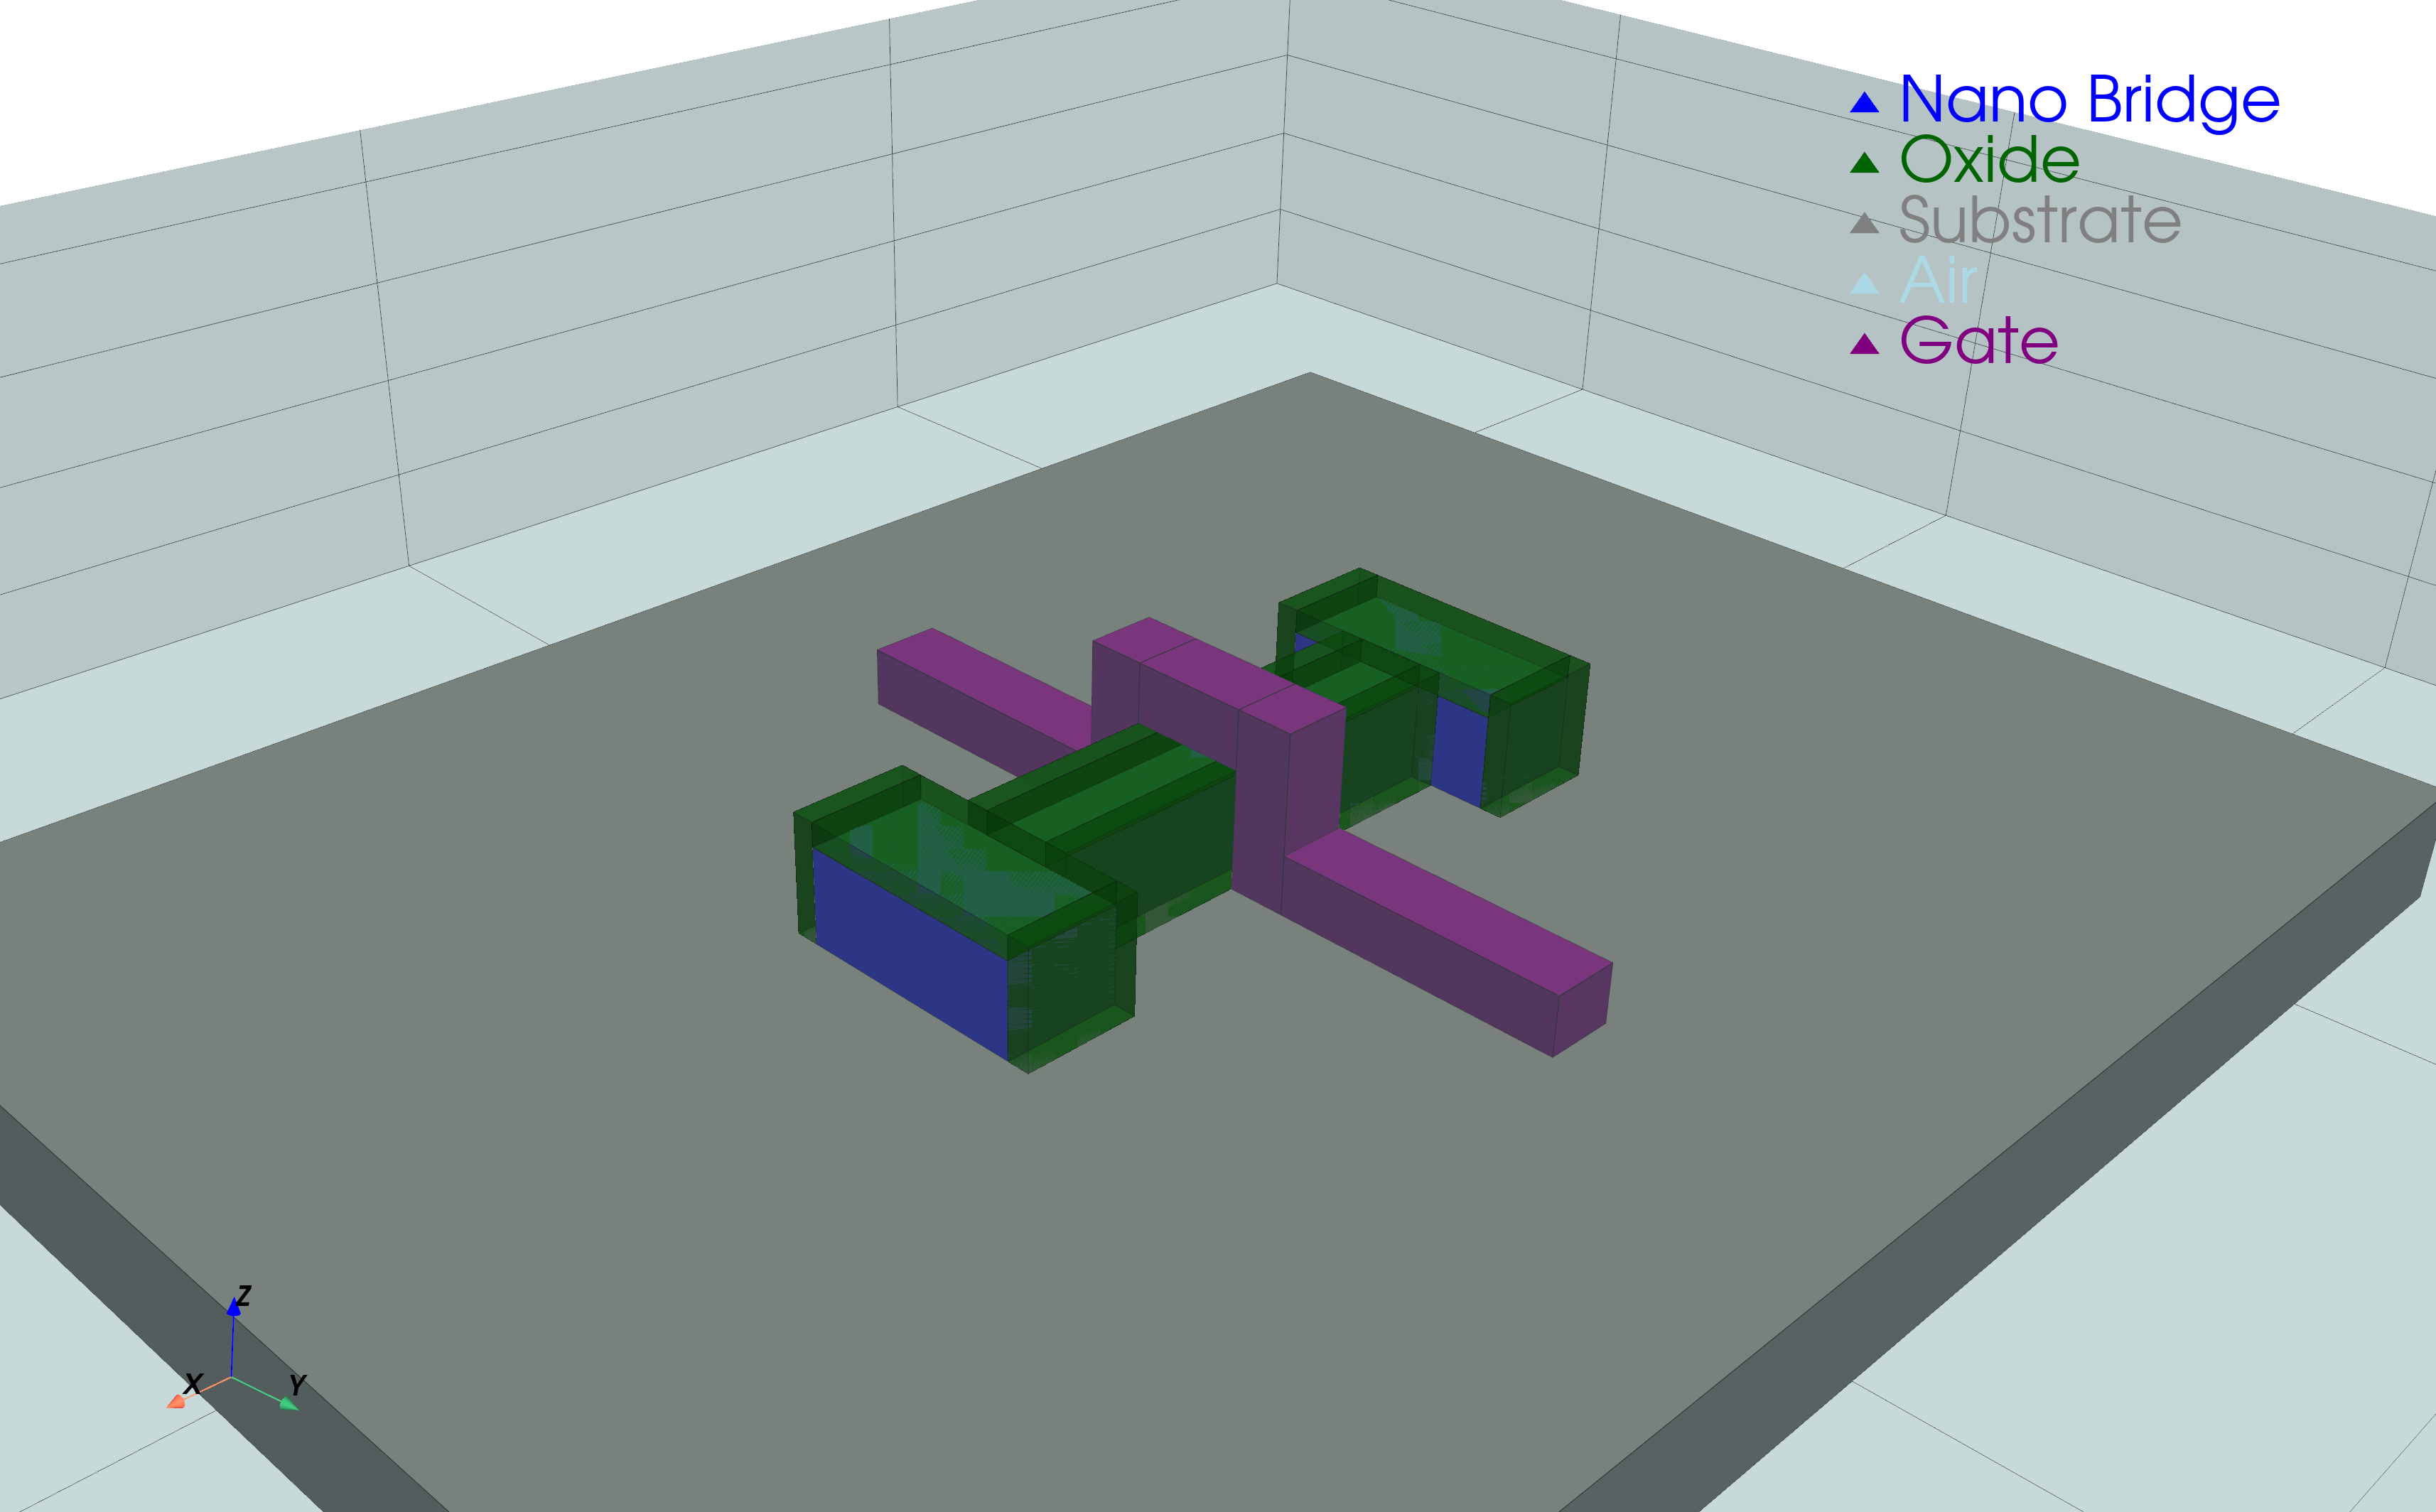
\includegraphics[width=1.0\linewidth]{images/el_1.png}
    \caption{Структура на которой показаны возможности программного задания модели. Есть возможность задавать нанопровод с утолщениями по краям (синий цвет), оксид на этом нанопроводе (зеленный цвет), а также завторный элетрод с оксидом на нем (фиолетовый цвет)}
    \label{fig:model}
\end{figure}

\begin{figure}[]
    \centering
    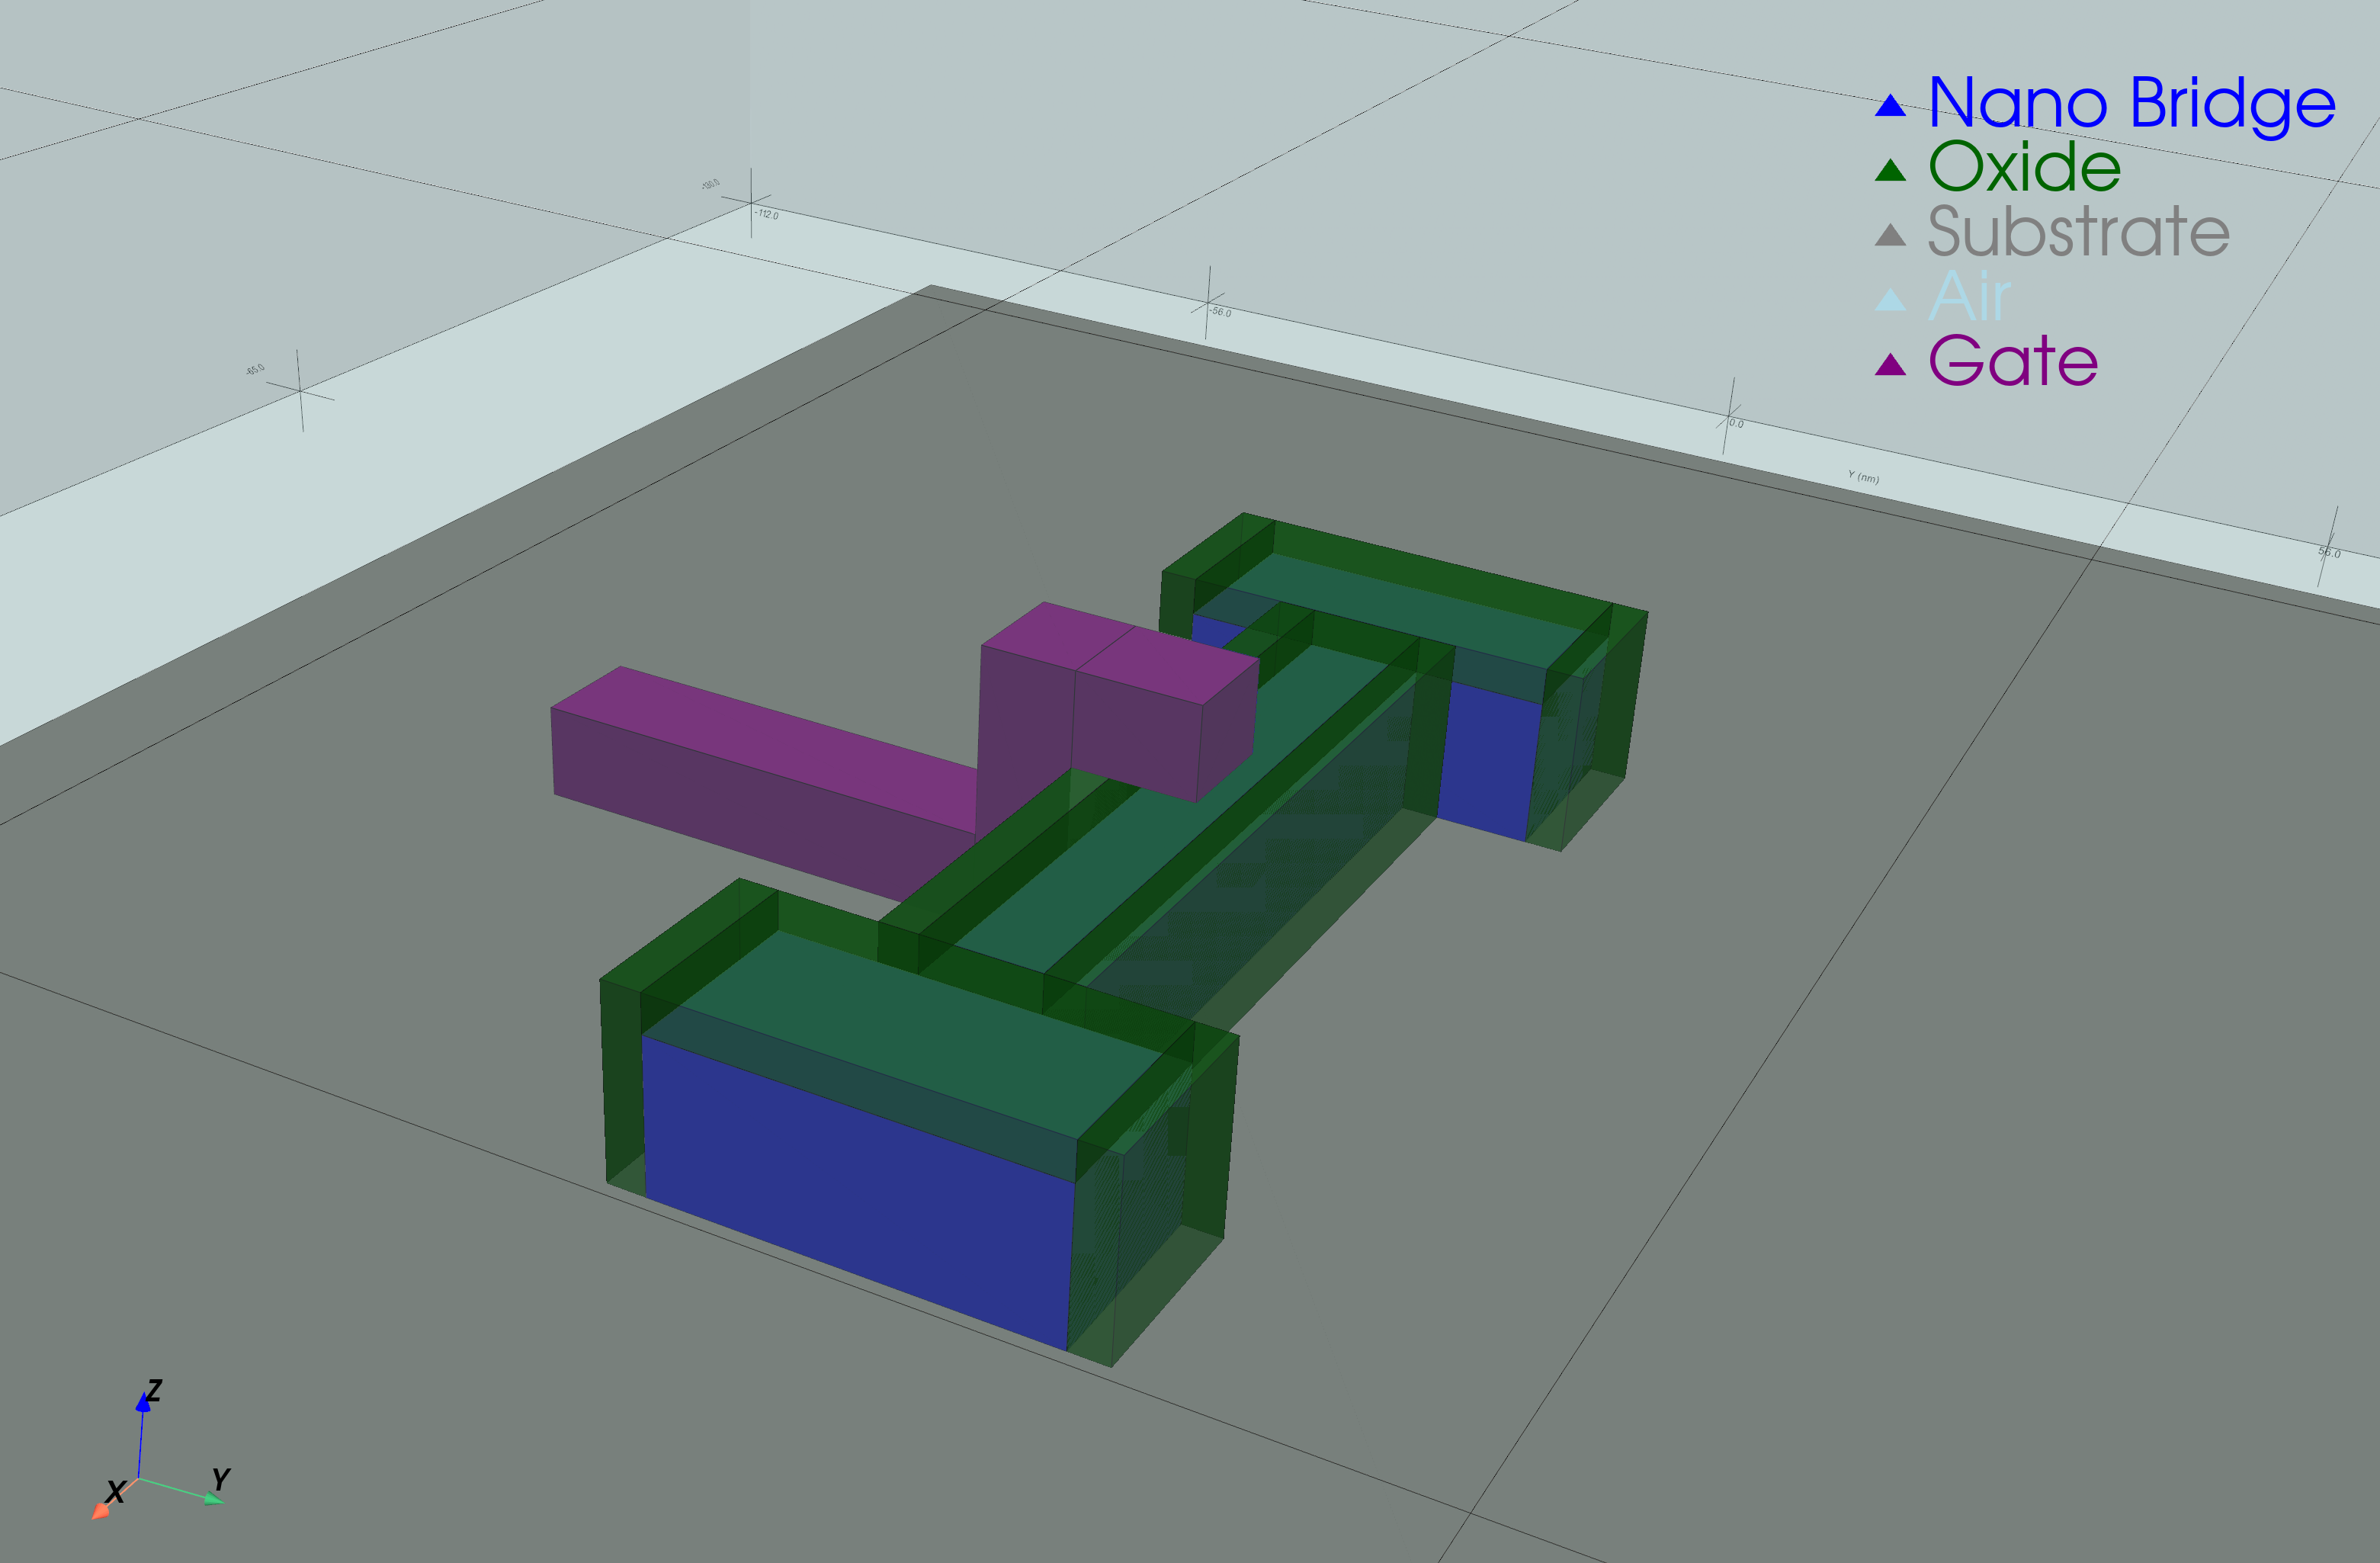
\includegraphics[width=1.0\linewidth]{images/gate_1_not_full.png}
    \caption{Пример с 1 затвором, который не полностью покрывает наномостик}
    \label{fig:model_3electrodes}
\end{figure}

\begin{figure}[]
    \centering
    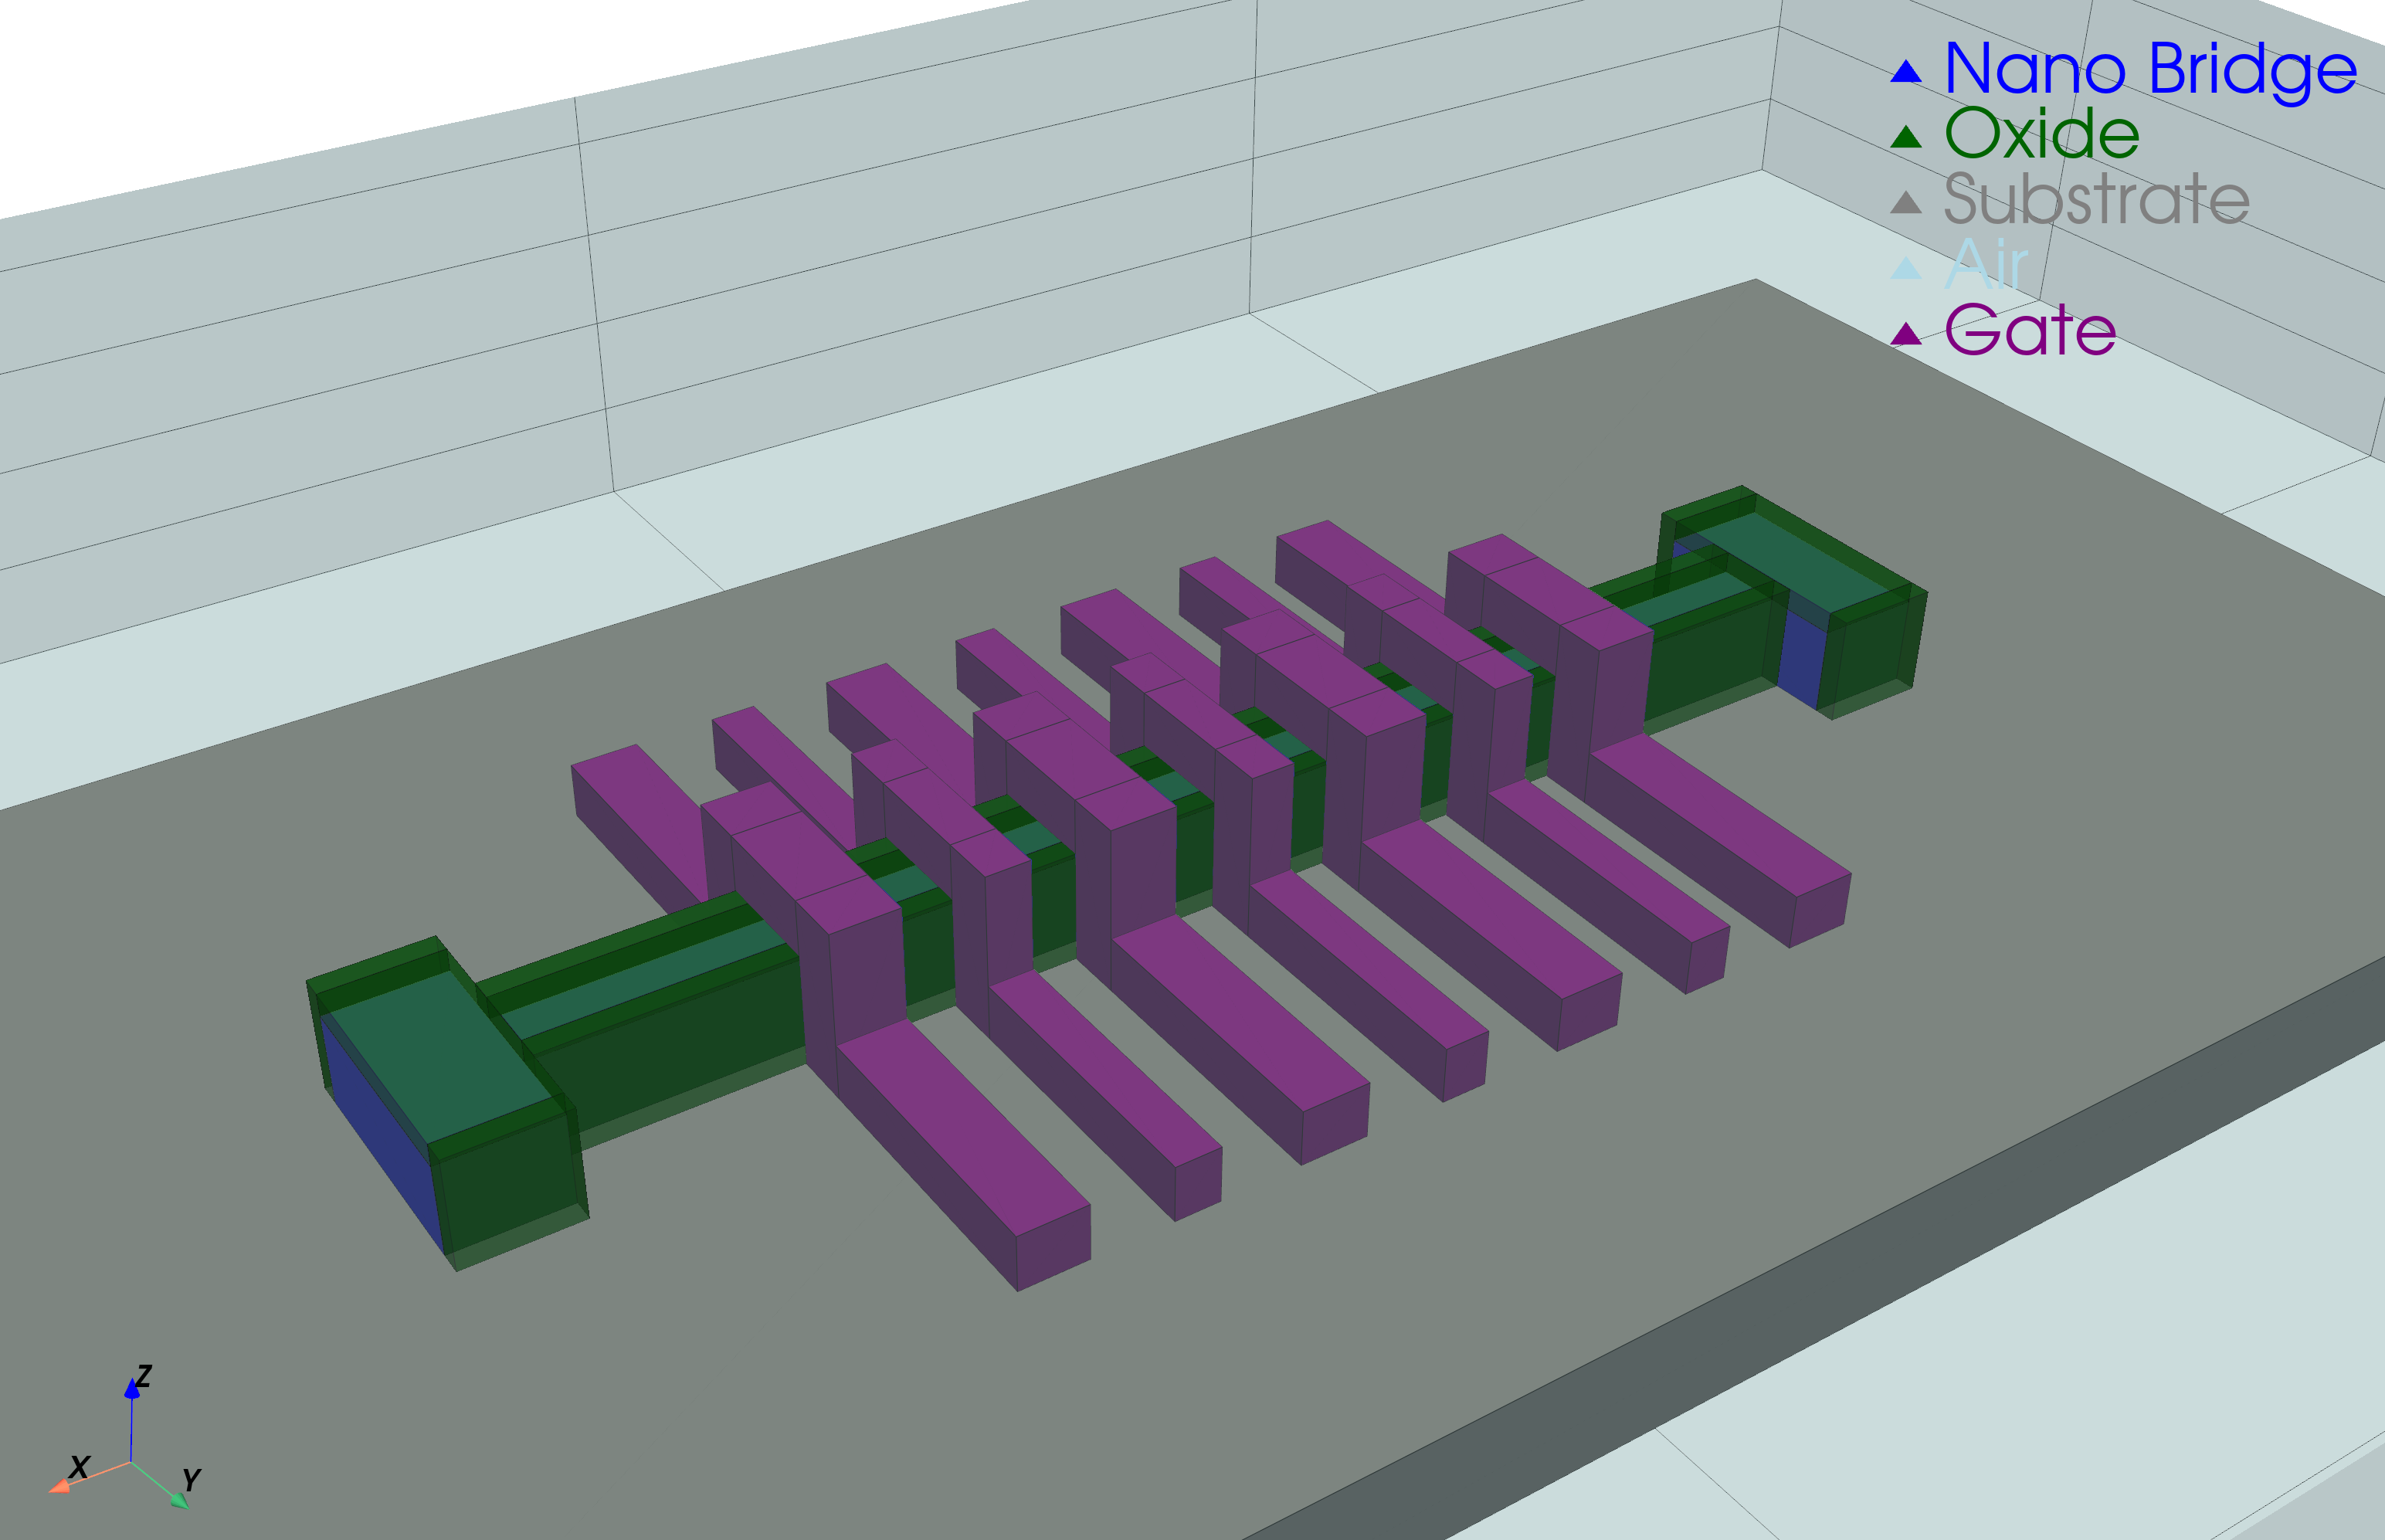
\includegraphics[width=1.0\linewidth]{images/many_el.png}
    \caption{Пример со множеством элетродов}
    \label{fig:model_many_electrodes}
\end{figure}


\section{Математическая модель и численный расчет электрического поля}

\subsection{Постановка задачи}
Расчет распределения электрического потенциала $\varphi$ в исследуемой наносистеме сводится к решению дифференциального уравнения для неоднородной диэлектрической среды в отсутствие свободных зарядов:
\begin{equation}
    \nabla \cdot (\varepsilon(x, y, z) \nabla \varphi) = 0,
\end{equation}
где $\varepsilon(x, y, z)$ — относительная диэлектрическая проницаемость среды в заданной точке пространства.

Для решения эллиптического уравнения (1) задаются граничные условия первого рода. На внешних границах расчетной области (воздушной среды) потенциал принимается равным нулю ($\varphi_{bnd} = 0$). На поверхностях и внутри объемов заданных электродов потенциал фиксируется согласно внешним приложенным напряжениям:
\begin{equation}
    \varphi\big|_{\Gamma_k} = V_k,
\end{equation}
где $\Gamma_k$ — область $k$-го электрода, $V_k$ — заданный потенциал.

Расчет вектора напряженности электрического поля $\mathbf{E}$ производится на основе найденного распределения потенциала:
\begin{equation}
    \mathbf{E} = -\nabla \varphi.
\end{equation}

\subsection{Численный метод решения}
Для численного решения уравнения (1) применялся метод конечных разностей на равномерной прямоугольной 3D-сетке. Расчетная область разбивается на узлы $(i, j, k)$. Поскольку среда является неоднородной, эффективная диэлектрическая проницаемость между соседними узлами рассчитывается как среднее арифметическое. Например, для оси $X$:
\begin{equation}
    \varepsilon_{i-1/2, j, k} = \frac{\varepsilon_{i, j, k} + \varepsilon_{i-1, j, k}}{2}, \quad 
    \varepsilon_{i+1/2, j, k} = \frac{\varepsilon_{i, j, k} + \varepsilon_{i+1, j, k}}{2}.
\end{equation}

Аппроксимация уравнения (1) по схеме крест приводит к следующему выражению для вычисления локального потенциала в центральном узле:
\begin{equation}
    \varphi_{i,j,k}^* = \frac{\sum \limits_{m \in S} \varepsilon_{m} \varphi_{m}}{\sum \limits_{m \in S} \varepsilon_{m}},
\end{equation}
где $S$ — множество шести соседних узлов по осям $X, Y, Z$, $\varepsilon_m$ — усредненная проницаемость между центральным и $m$-м узлом, $\varphi_m$ — значение потенциала в соседнем узле. 

Система линейных алгебраических уравнений, получаемая после конечно-разностной аппроксимации, решалась итерационным методом последовательной верхней релаксации (SOR --- Successive Over-Relaxation). Пересчет значений потенциала на $n+1$ итерации производился по формуле:
\begin{equation}
    \varphi_{i,j,k}^{(n+1)} = \varphi_{i,j,k}^{(n)} + \omega \left( \varphi_{i,j,k}^* - \varphi_{i,j,k}^{(n)} \right),
\end{equation}
где $\omega \in (1, 2)$ — параметр релаксации, ускоряющий сходимость.

Итерационный процесс завершается при выполнении условия малости максимального приращения на всем поле:
\begin{equation}
    \max |\varphi^{(n+1)} - \varphi^{(n)}| < \delta,
\end{equation}
где $\delta$ — заданная погрешность (критерий сходимости, $\delta = 0.5$).

\subsection{Программная реализация}
Программный комплекс для моделирования электрического поля реализован на языке Python. В рамках реализации создана объектно-ориентированная архитектура, выполняющая следующие этапы:
\begin{itemize}
    \item \textbf{Генерация вычислительной сетки:} построение трехмерной матрицы координат по габаритам внешней воздушной среды.
    \item \textbf{Инициализация карты материалов:} распределение диэлектрических проницаемостей по узлам сетки на основе геометрических пересечений.
    \item \textbf{Формирование маски граничных условий:} выделение узлов сетки, принадлежащих электродам и внешним границам, для фиксации потенциалов на этапе итерационного расчета.
\end{itemize}

 Процесс расчета компонентов вектора напряженности электрического поля проводился методом центральных разностей. 

Результаты вычислений, включающие трехмерные матрицы потенциала и напряженности поля, сериализуются и сохраняются для последующего этапа визуализации и обработки.

\begin{figure}[!ht]
    \centering
    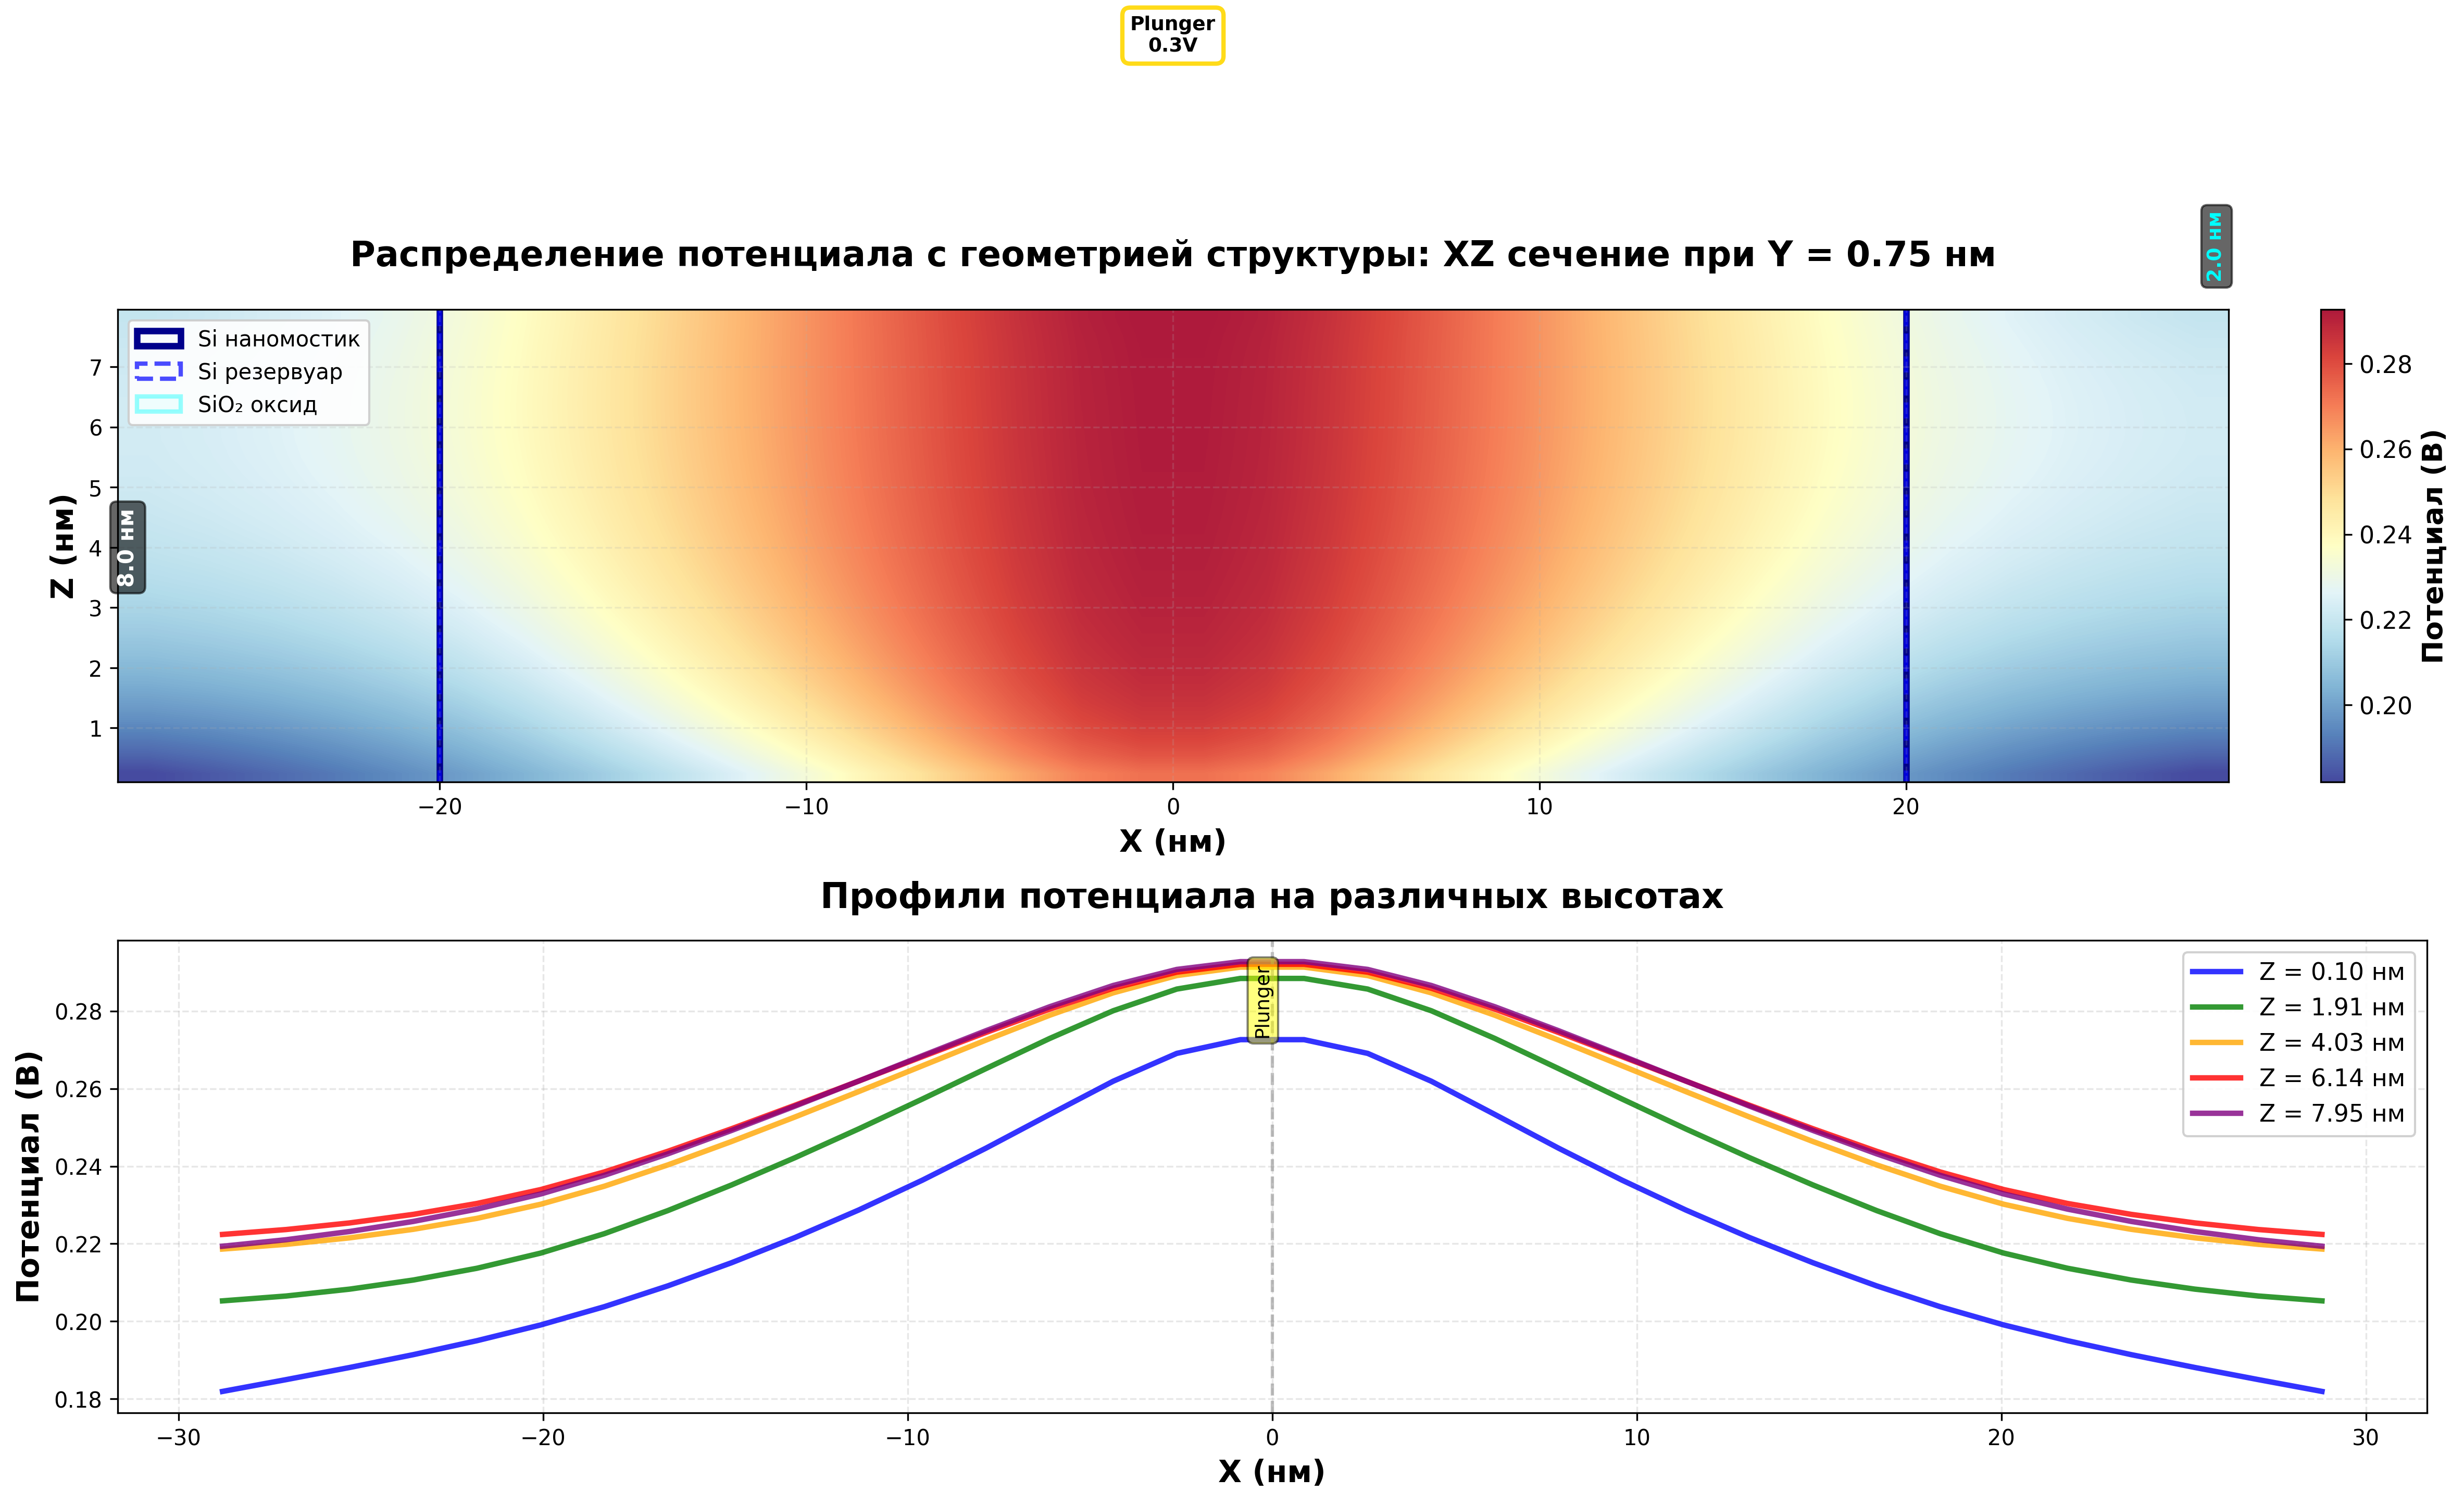
\includegraphics[width=0.95\linewidth,keepaspectratio]{images/nanobridge_cross_section_1qd.png}
    \caption{Распределение электростатического потенциала в поперечном сечении наномостика для конфигурации одиночной квантовой точки.
    Структура содержит один затворный электрод с потенциалом 0.3~В, расположенный в центре наномостика.}
    \label{fig:1qd}
\end{figure}

\begin{figure}[!ht]
    \centering
    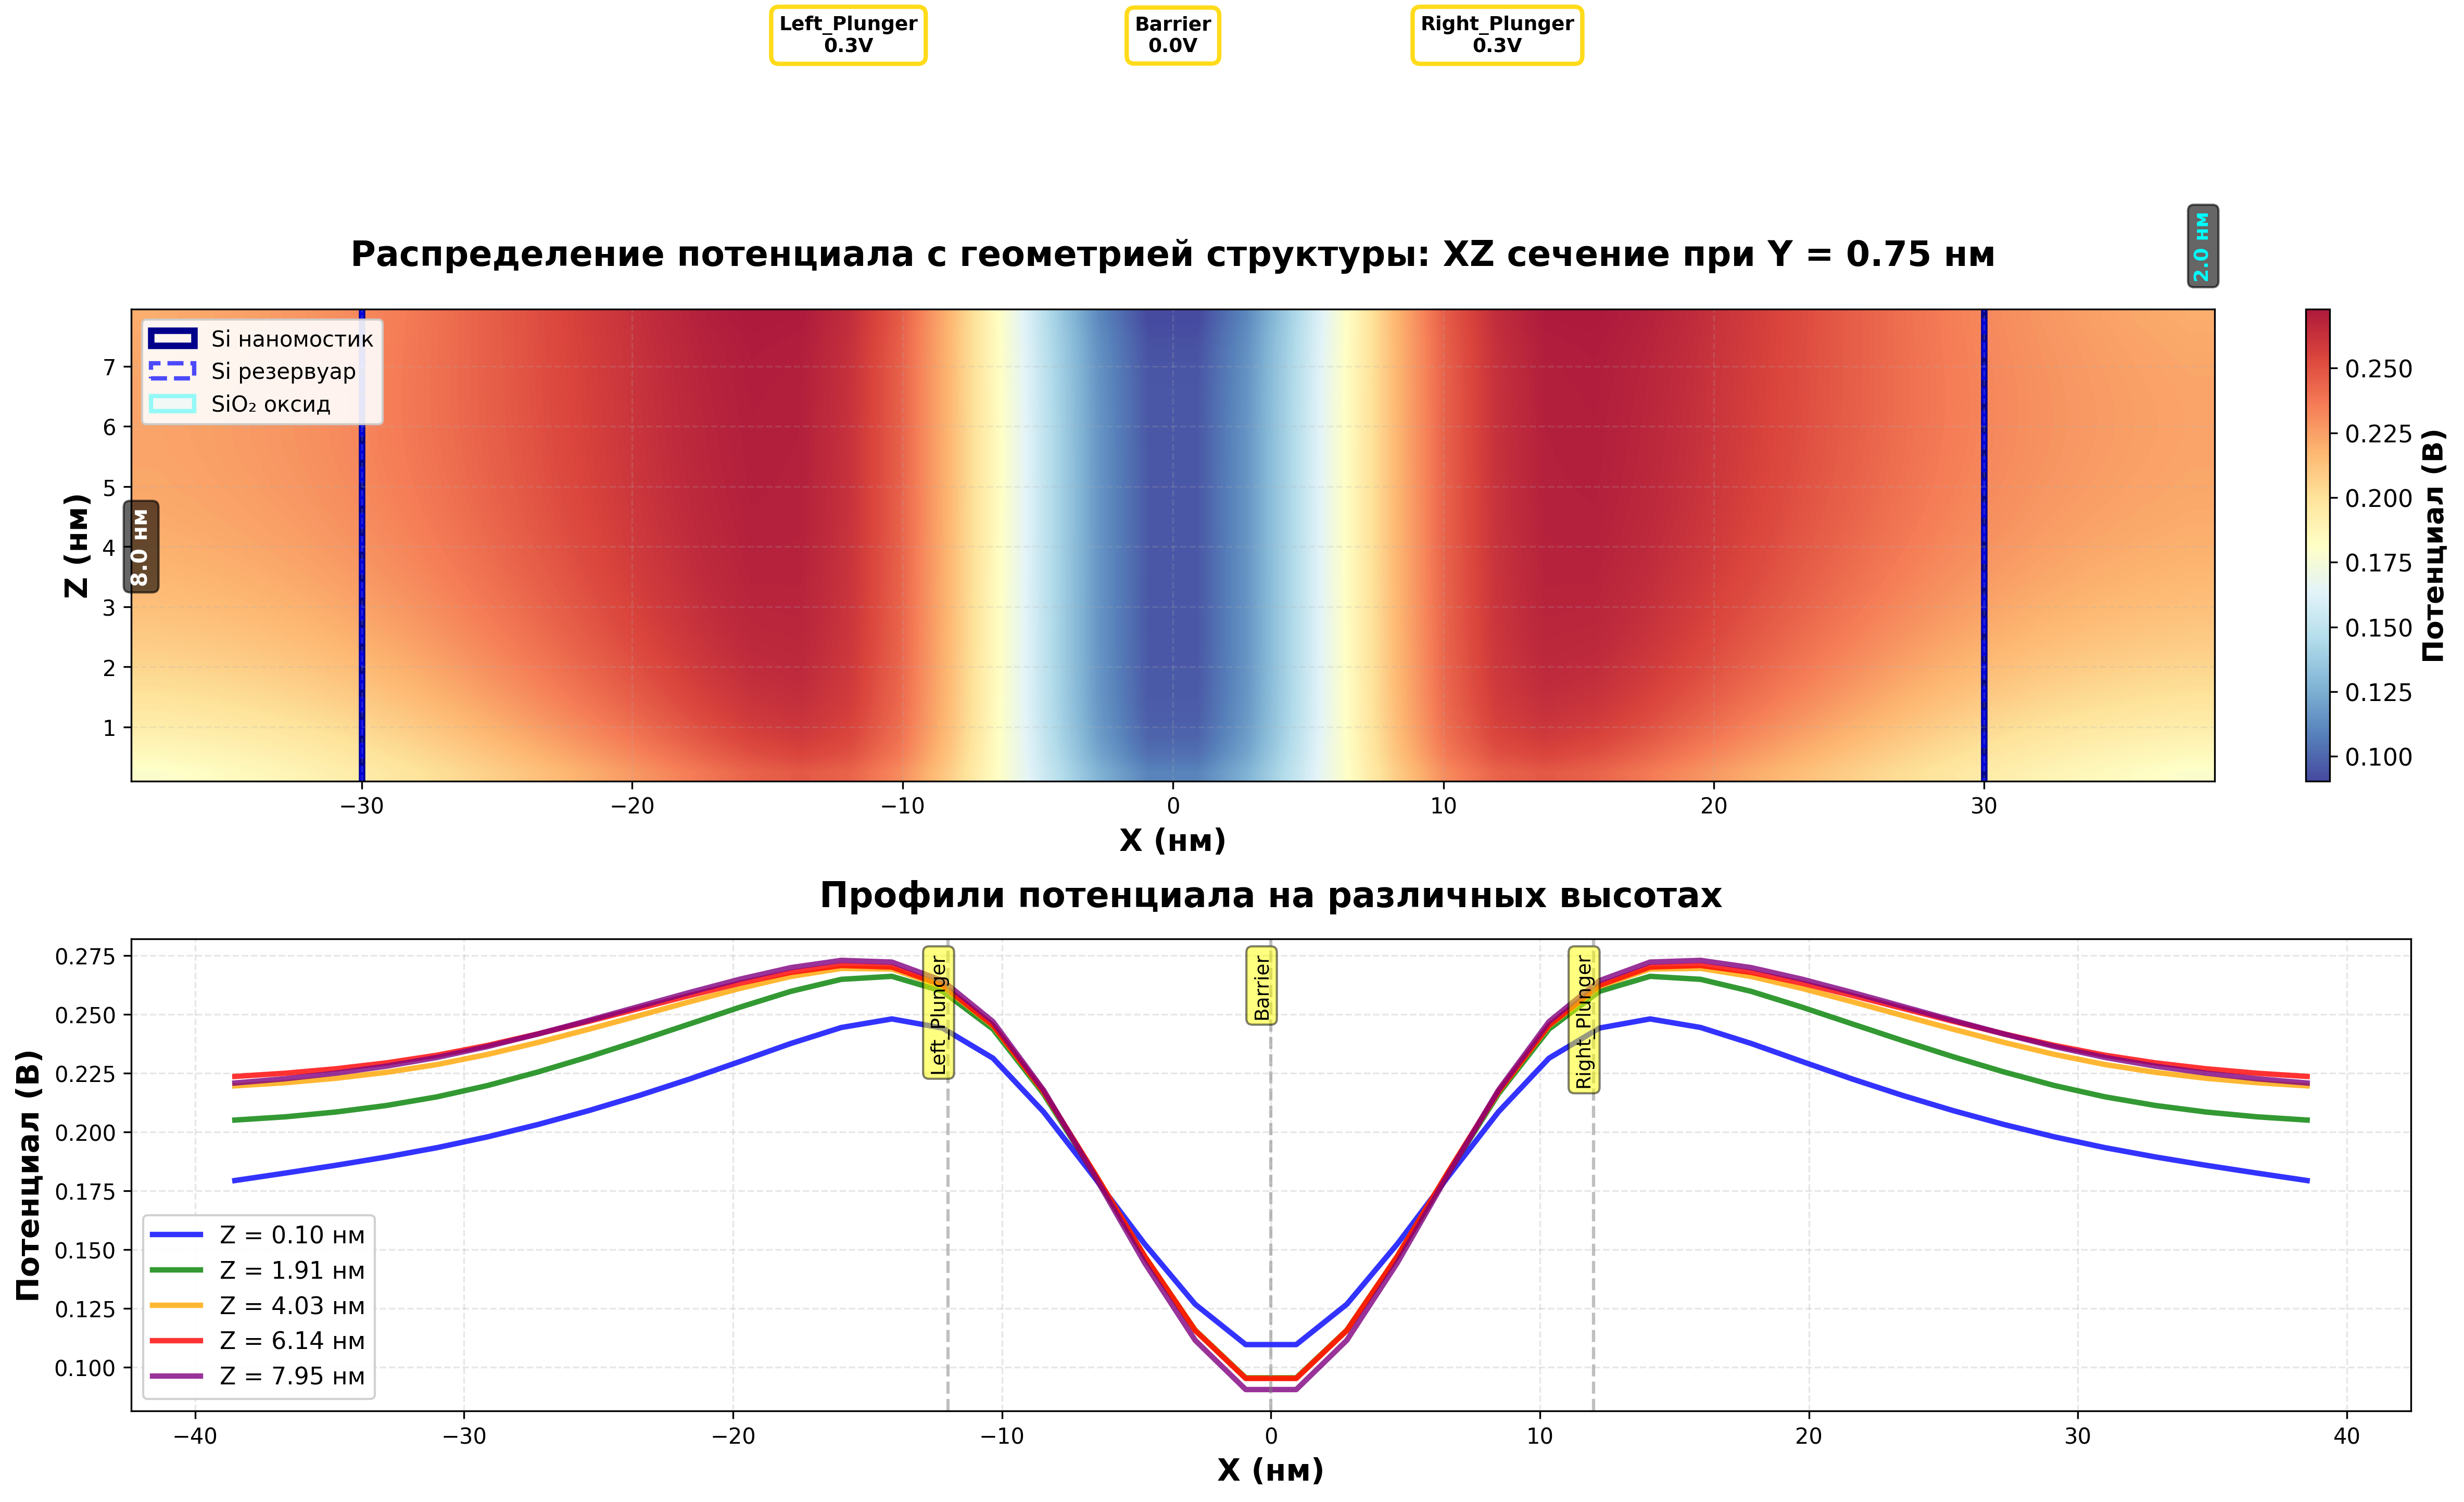
\includegraphics[width=0.95\linewidth,keepaspectratio]{images/nanobridge_cross_section_2qd.png}
    \caption{Распределение электростатического потенциала в поперечном сечении
    наномостика для конфигурации двойной квантовой точки (Double Quantum Dot)
    по архитектуре Loss-DiVincenzo. Структура содержит три затворных электрода:
     левый и правый плунжерные затворы (Left/Right Plunger) с потенциалом 0.3~В
     и центральный барьерный затвор (Barrier) с потенциалом 0~В.}
    \label{fig:2qd}
\end{figure}


\section{Квантово-механическая модель и расчет энергетического спектра}

\subsection{Постановка задачи}
Распределение электрического потенциала $\varphi(x, y, z)$, полученное на предыдущем этапе моделирования, формирует профиль потенциальной энергии для носителей заряда. Для нахождения возможных энергетических состояний электрона в области наномостика необходимо решить стационарное трехмерное уравнение Шрёдингера:
\begin{equation}
    \hat{H} \psi(x,y,z) = E \psi(x,y,z),
\end{equation}
где $\hat{H}$ — гамильтониан системы, $\psi(x,y,z)$ — волновая функция электрона, $E$ — искомые собственные значения энергии. 

Гамильтониан в рамках приближения эффективной массы имеет вид:
\begin{equation}
    \hat{H} = -\frac{\hbar^2}{2 m^*} \nabla^2 + U(x,y,z),
\end{equation}
где $\hbar$ — приведенная постоянная Планка, $m^*$ — эффективная масса электрона в материале полупроводника. Потенциальная энергия электрона $U(x,y,z)$ связана с рассчитанным электростатическим потенциалом соотношением:
\begin{equation}
    U(x,y,z) = -e \cdot \varphi(x,y,z).
\end{equation}
В вычислительном алгоритме расчеты проводятся в электрон-вольтах (эВ), вследствие чего численное значение потенциальной энергии берется со знаком минус от значения электрического потенциала в вольтах.

\subsection{Дискретизация гамильтониана}
Для численного решения уравнения (8) применялся метод конечных разностей. Оператор Лапласа $\nabla^2$ аппроксимировался центральными разностями второго порядка на той же пространственной сетке с шагами $\Delta x, \Delta y, \Delta z$:
\begin{equation}
    \frac{\partial^2 \psi}{\partial x^2} \approx \frac{\psi_{i+1,j,k} - 2\psi_{i,j,k} + \psi_{i-1,j,k}}{\Delta x^2}
\end{equation}
и аналогично для осей $Y$ и $Z$.

При подстановке конечно-разностных производных уравнение Шрёдингера трансформируется в алгебраическую проблему собственных значений для разреженной матрицы:
\begin{equation}
    \mathbf{H} \mathbf{\Psi} = E \mathbf{\Psi},
\end{equation}
где вектор $\mathbf{\Psi}$ размерности $N = n_x \times n_y \times n_z$ содержит значения волновой функции в узлах сетки.

Матрица гамильтониана $\mathbf{H}$ является симметричной, ленточной (имеет блочно-трехдиагональную структуру на основе 7-точечного шаблона). На главной диагонали матрицы располагаются суммы кинетического члена и локальной потенциальной энергии:
\begin{equation}
    H_{p,p} = \frac{\hbar^2}{2 m^*} \left( \frac{2}{\Delta x^2} + \frac{2}{\Delta y^2} + \frac{2}{\Delta z^2} \right) + U_{i,j,k},
\end{equation}
где индекс $p$ — сквозной (линейный) индекс узла сетки. Внедиагональные элементы, соответствующие связям с соседними узлами, равны $-\frac{\hbar^2}{2 m^* \Delta \alpha^2}$, где $\alpha \in \{x, y, z\}$.

\subsection{Вычислительные аспекты и программная реализация}
Решение задачи на собственные значения для 3D-сеток требует выделения значительных вычислительных ресурсов. Для оптимизации процесса был реализован следующий пайплайн:

\begin{enumerate}
    \item \textbf{Локализация области вычислений.} На основе геометрической конфигурации наносистемы глобальное поле потенциала программно обрезается. Из рассмотрения исключаются области диэлектрика и внешних электродов, поскольку вероятность нахождения электрона в них пренебрежимо мала. Это на несколько порядков уменьшает размерность матрицы $\mathbf{H}$ без потери физического смысла задачи.
    
    \item \textbf{Сборка разреженной матрицы.} Описание матрицы гамильтониана выполняется в формате сжатых разреженных строк с использованием библиотек подпрограмм \texttt{SciPy}. Это позволяет хранить в памяти компьютера только 7 ненулевых диагоналей матрицы вместо всего объема $N^2$.
    
    \item \textbf{Поиск собственных значений.} Физический интерес представляют лишь несколько самых нижних энергетических уровней (основное и первые возбужденные состояния). Поэтому полная диагонализация матрицы не производится. Применяется алгоритм Ланцоша/Арнольди.
    
    \item \textbf{Представление результатов.} Найденные собственные векторы преобразуются обратно в трехмерные тензоры. Для каждой волновой функции вычисляется и нормируется плотность вероятности нахождения электрона $\rho = |\psi|^2$:
    \begin{equation}
        \sum_{i,j,k} |\psi_{i,j,k}|^2 \Delta x \Delta y \Delta z = 1.
    \end{equation}
    Квантованные уровни энергии $E_n$ образуют энергетический спектр системы.
\end{enumerate}

\begin{figure}[!p]
    \centering
    \begin{subfigure}[b]{0.95\textwidth}
        \centering
        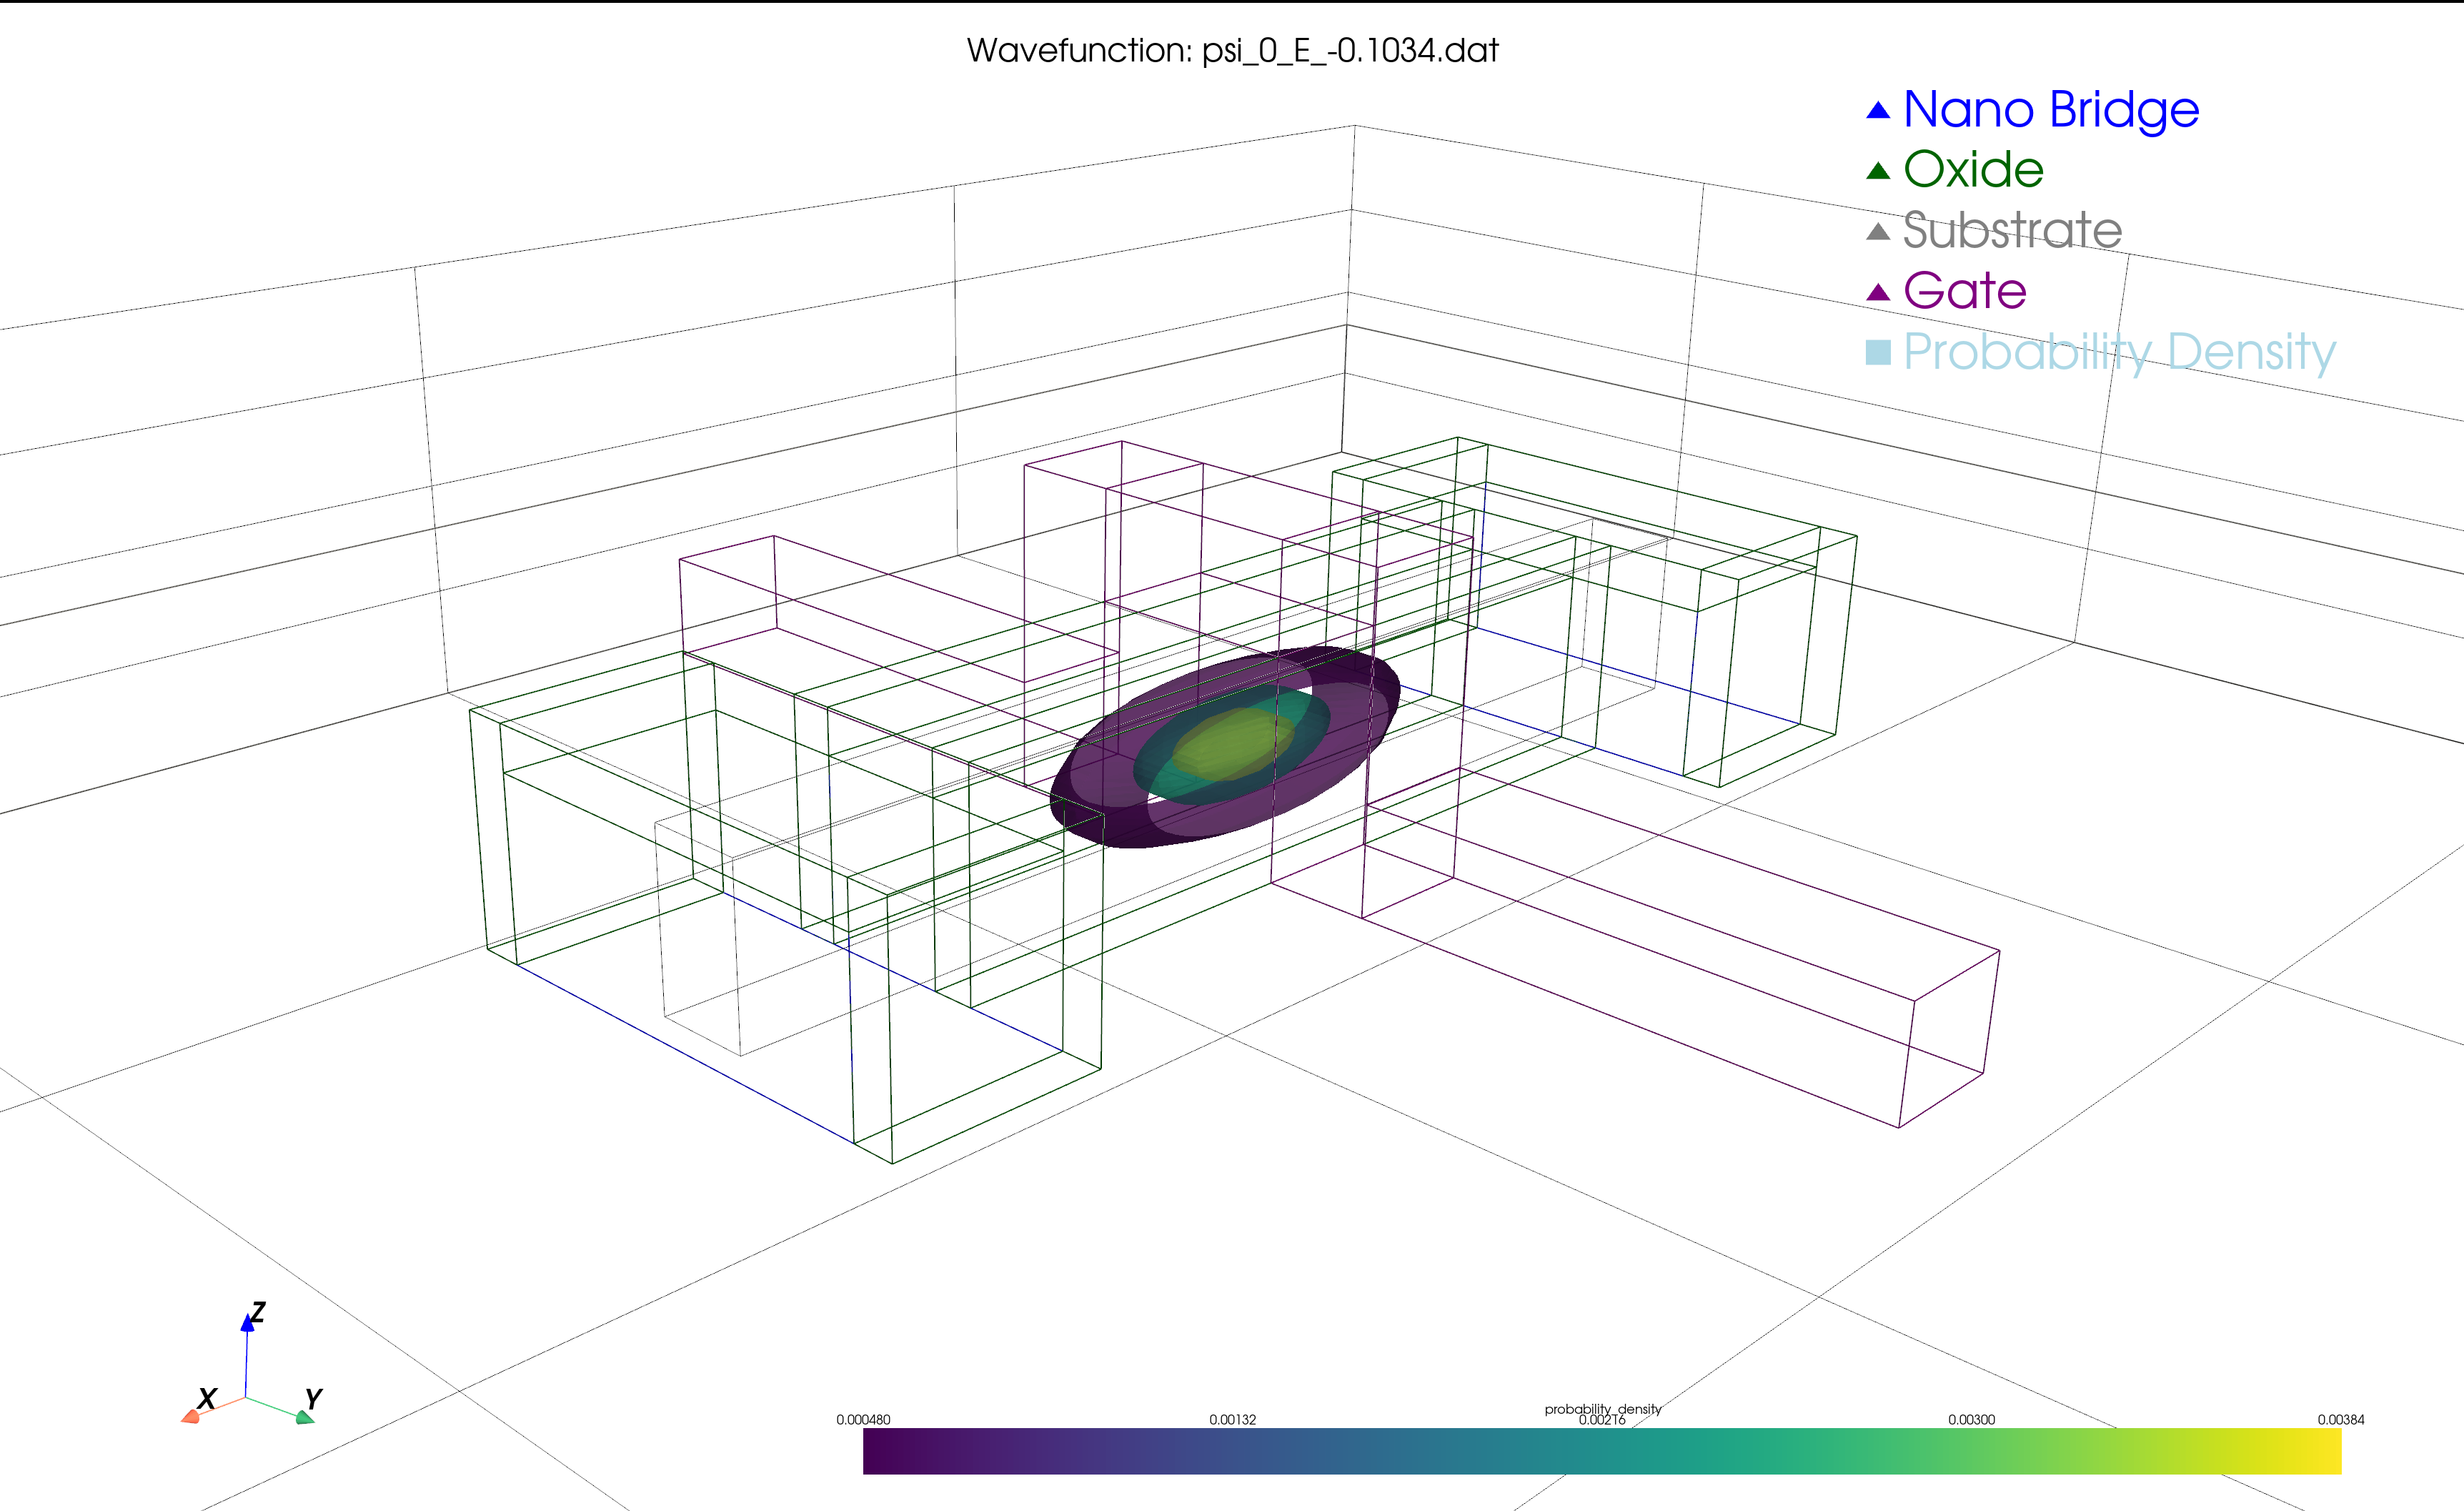
\includegraphics[width=\textwidth,keepaspectratio]{images/wf_1qd_E0.png}
        \caption{Одиночная квантовая точка (Single QD)}
        \label{fig:wf_1qd_E0}
    \end{subfigure}
    
    \vspace{1em}
    
    \begin{subfigure}[b]{0.95\textwidth}
        \centering
        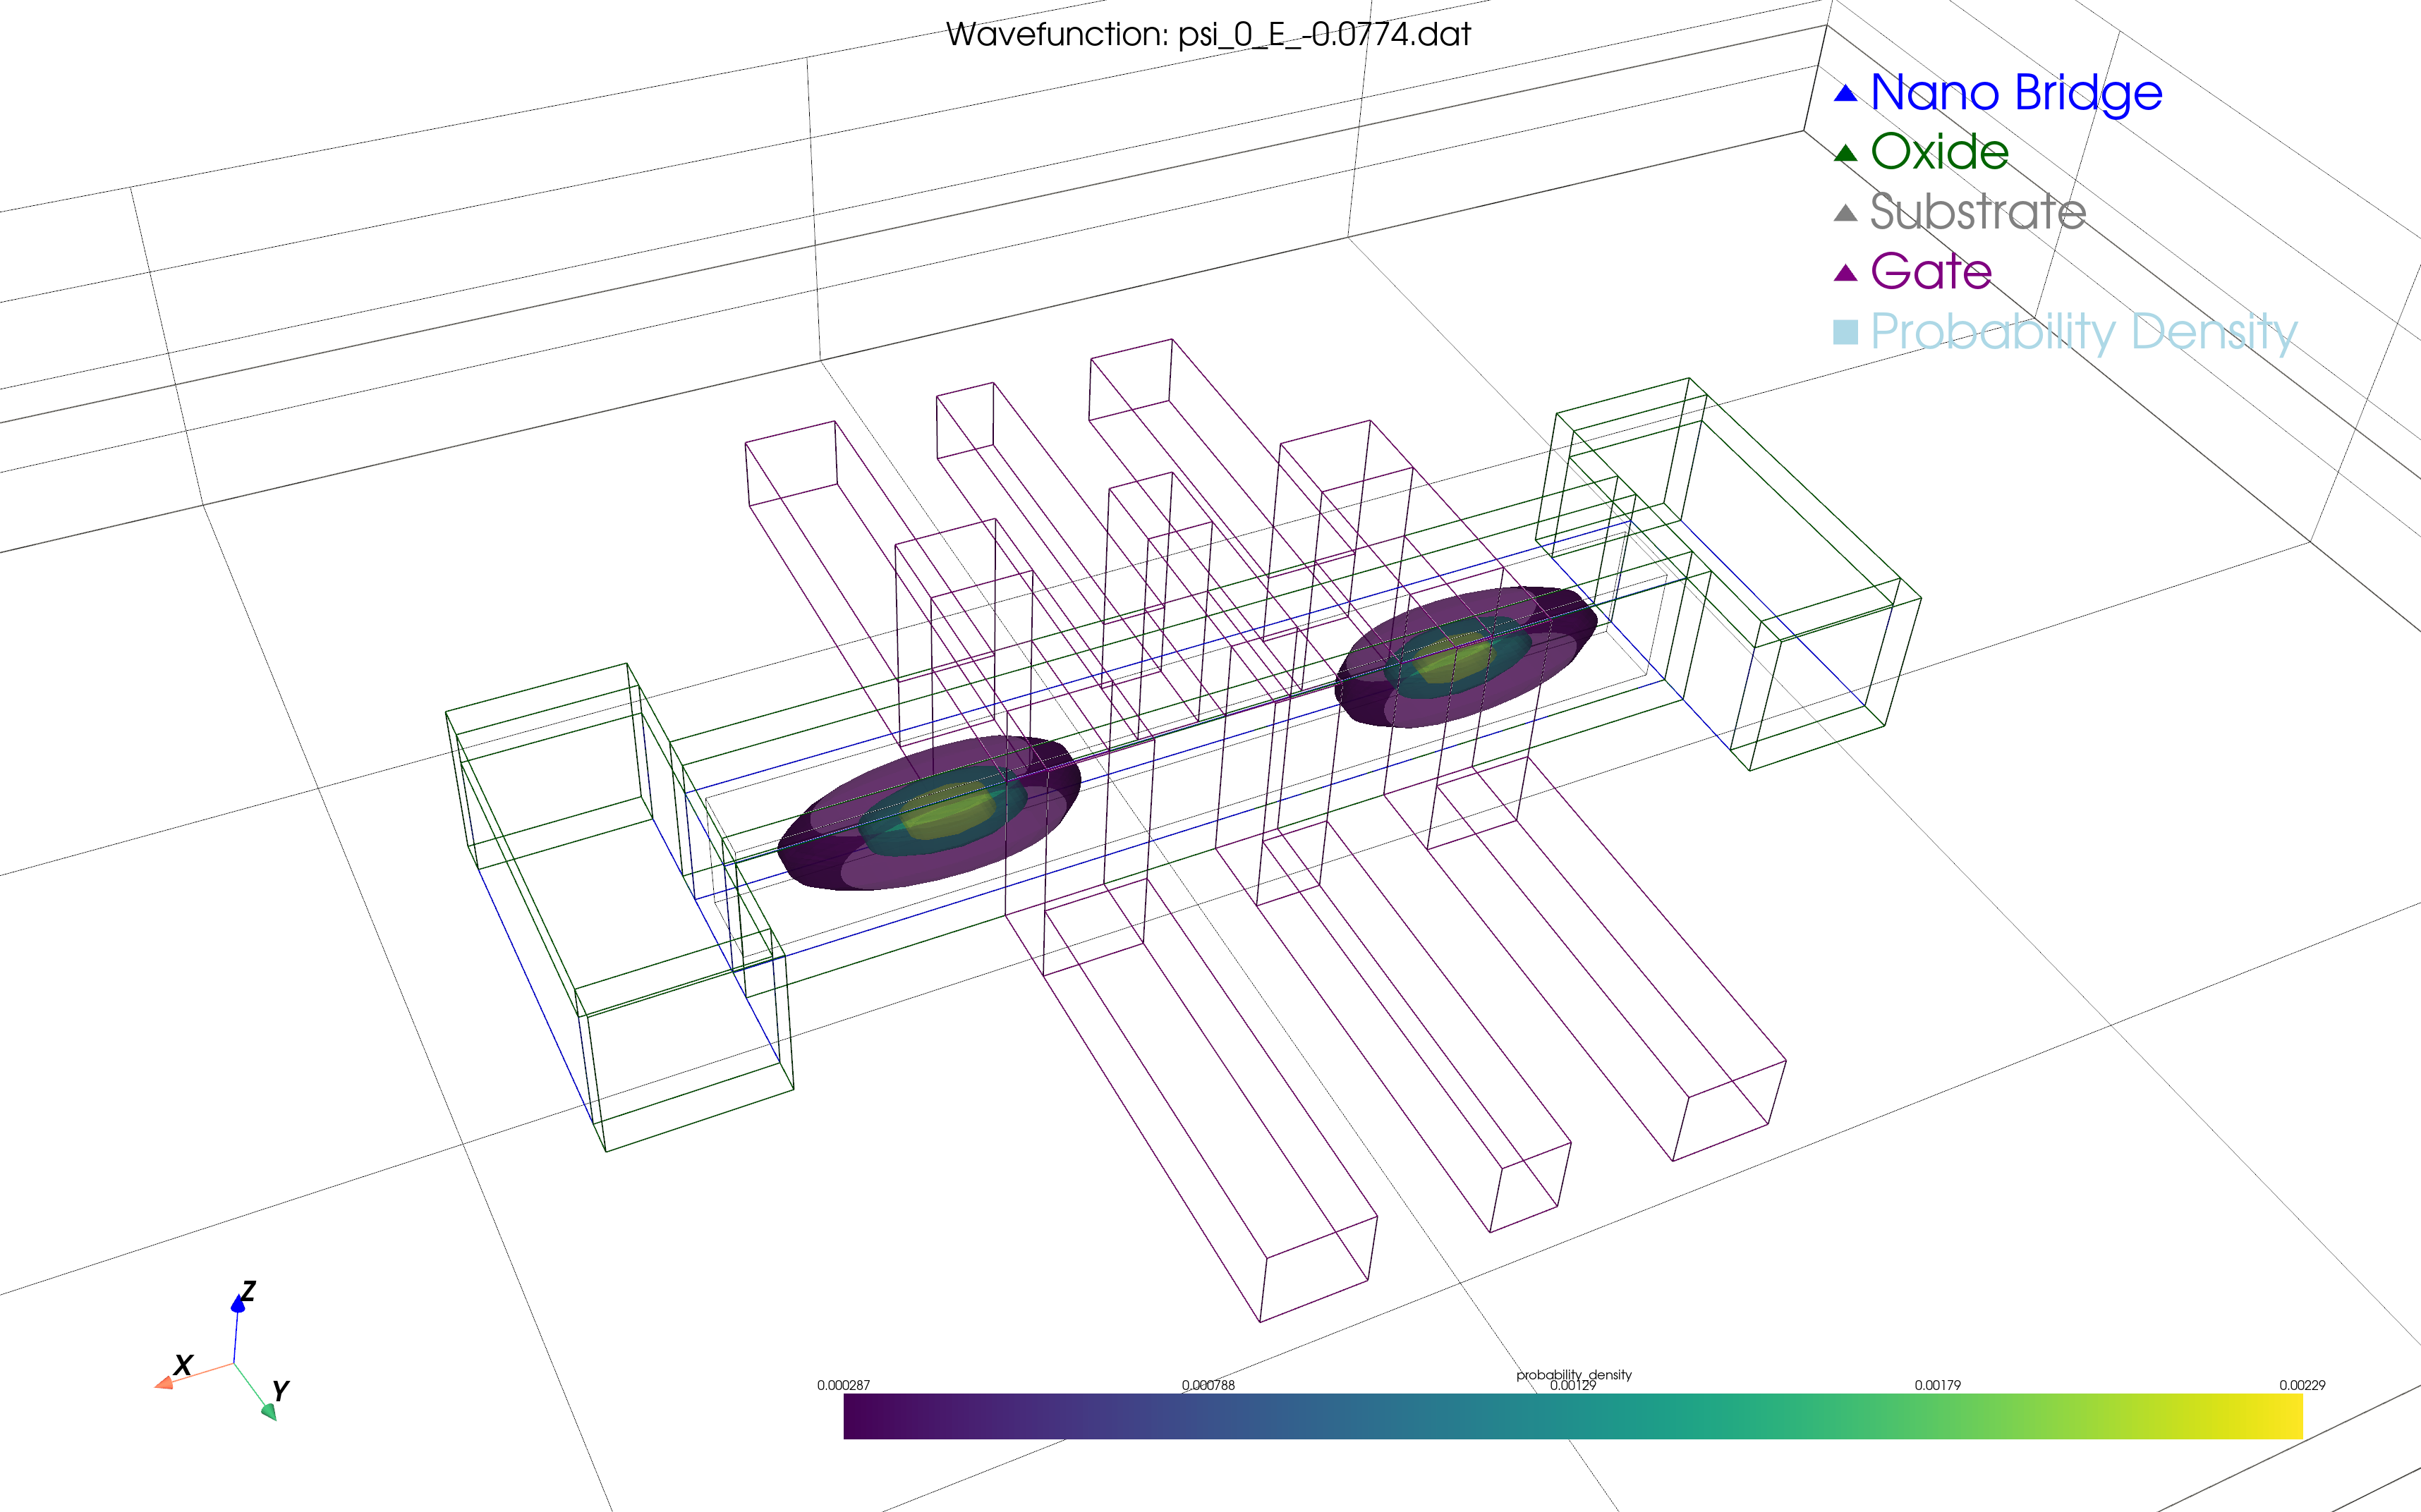
\includegraphics[width=\textwidth,keepaspectratio]{images/wf_2qd_E0.png}
        \caption{Двойная квантовая точка (Double QD)}
        \label{fig:wf_2qd_E0}
    \end{subfigure}
    
    \caption{Визуализация волновых функций основного состояния ($E_0$) для различных конфигураций квантовых точек. 
    Показано пространственное распределение плотности вероятности $|\psi_0|^2$ нахождения электрона в наномостике. (a) Для конфигурации с одним затворным электродом наблюдается локализация электрона в единственной потенциальной яме. (b) Для архитектуры Loss-DiVincenzo с тремя электродами.}
    \label{fig:wf_comparison}
\end{figure}

\chapter{Результаты расчетов для различных структур}

В данной главе представлены результаты численного моделирования энергетического спектра 
и волновых функций для различных конфигураций наведенных квантовых точек в кремниевых 
наноструктурах. Расчеты выполнены с использованием разработанной модели, описанной в главе 3.

Исследованы следующие архитектуры:
\begin{enumerate}
    \item Одиночная квантовая точка — базовая конфигурация с одним плунжерным затвором
    \item Двойная квантовая точка — архитектура с тремя затворами
    \item Линейный массив квантовых точек — конфигурация для реализации спинового шатла
\end{enumerate}

Для каждой структуры проанализированы:
\begin{itemize}
    \item Распределение электростатического потенциала
    \item Энергетический спектр основных и возбужденных состояний
    \item Зависимость параметров от напряжений на затворах
\end{itemize}

\section{Одиночная квантовая точка}

\subsection{Геометрия и параметры структуры}

\begin{itemize}
    \item \textbf{Кремниевый наномостик:} длина 200 нм, ширина 50 нм, высота 10 нм
    \item \textbf{Плунжерный затвор:} ширина 50 нм, расположен в центре наномостика
    \item \textbf{Оксидный слой:} толщина 5 нм между затвором и наномостиком
    \item \textbf{Резервуары:} расположены по краям наномостика для загрузки электронов
\end{itemize}

Материальные параметры:
\begin{itemize}
    \item Эффективная масса электрона в Si: $m^* = 0.19 \, m_e$
    \item Диэлектрическая проницаемость Si: $\varepsilon_{Si} = 11.7$
    \item Диэлектрическая проницаемость SiO$_2$: $\varepsilon_{SiO_2} = 3.9$
\end{itemize}

\subsection{Электростатический потенциал}

На рисунке \ref{fig:1qd_main} представлено распределение электростатического потенциала 
в поперечном сечении наномостика. 
При приложении положительного напряжения $V_P = 0.3$ В к плунжерному затвору 
в центральной области наномостика формируется потенциальная яма.

\begin{figure}[!ht]
    \centering
    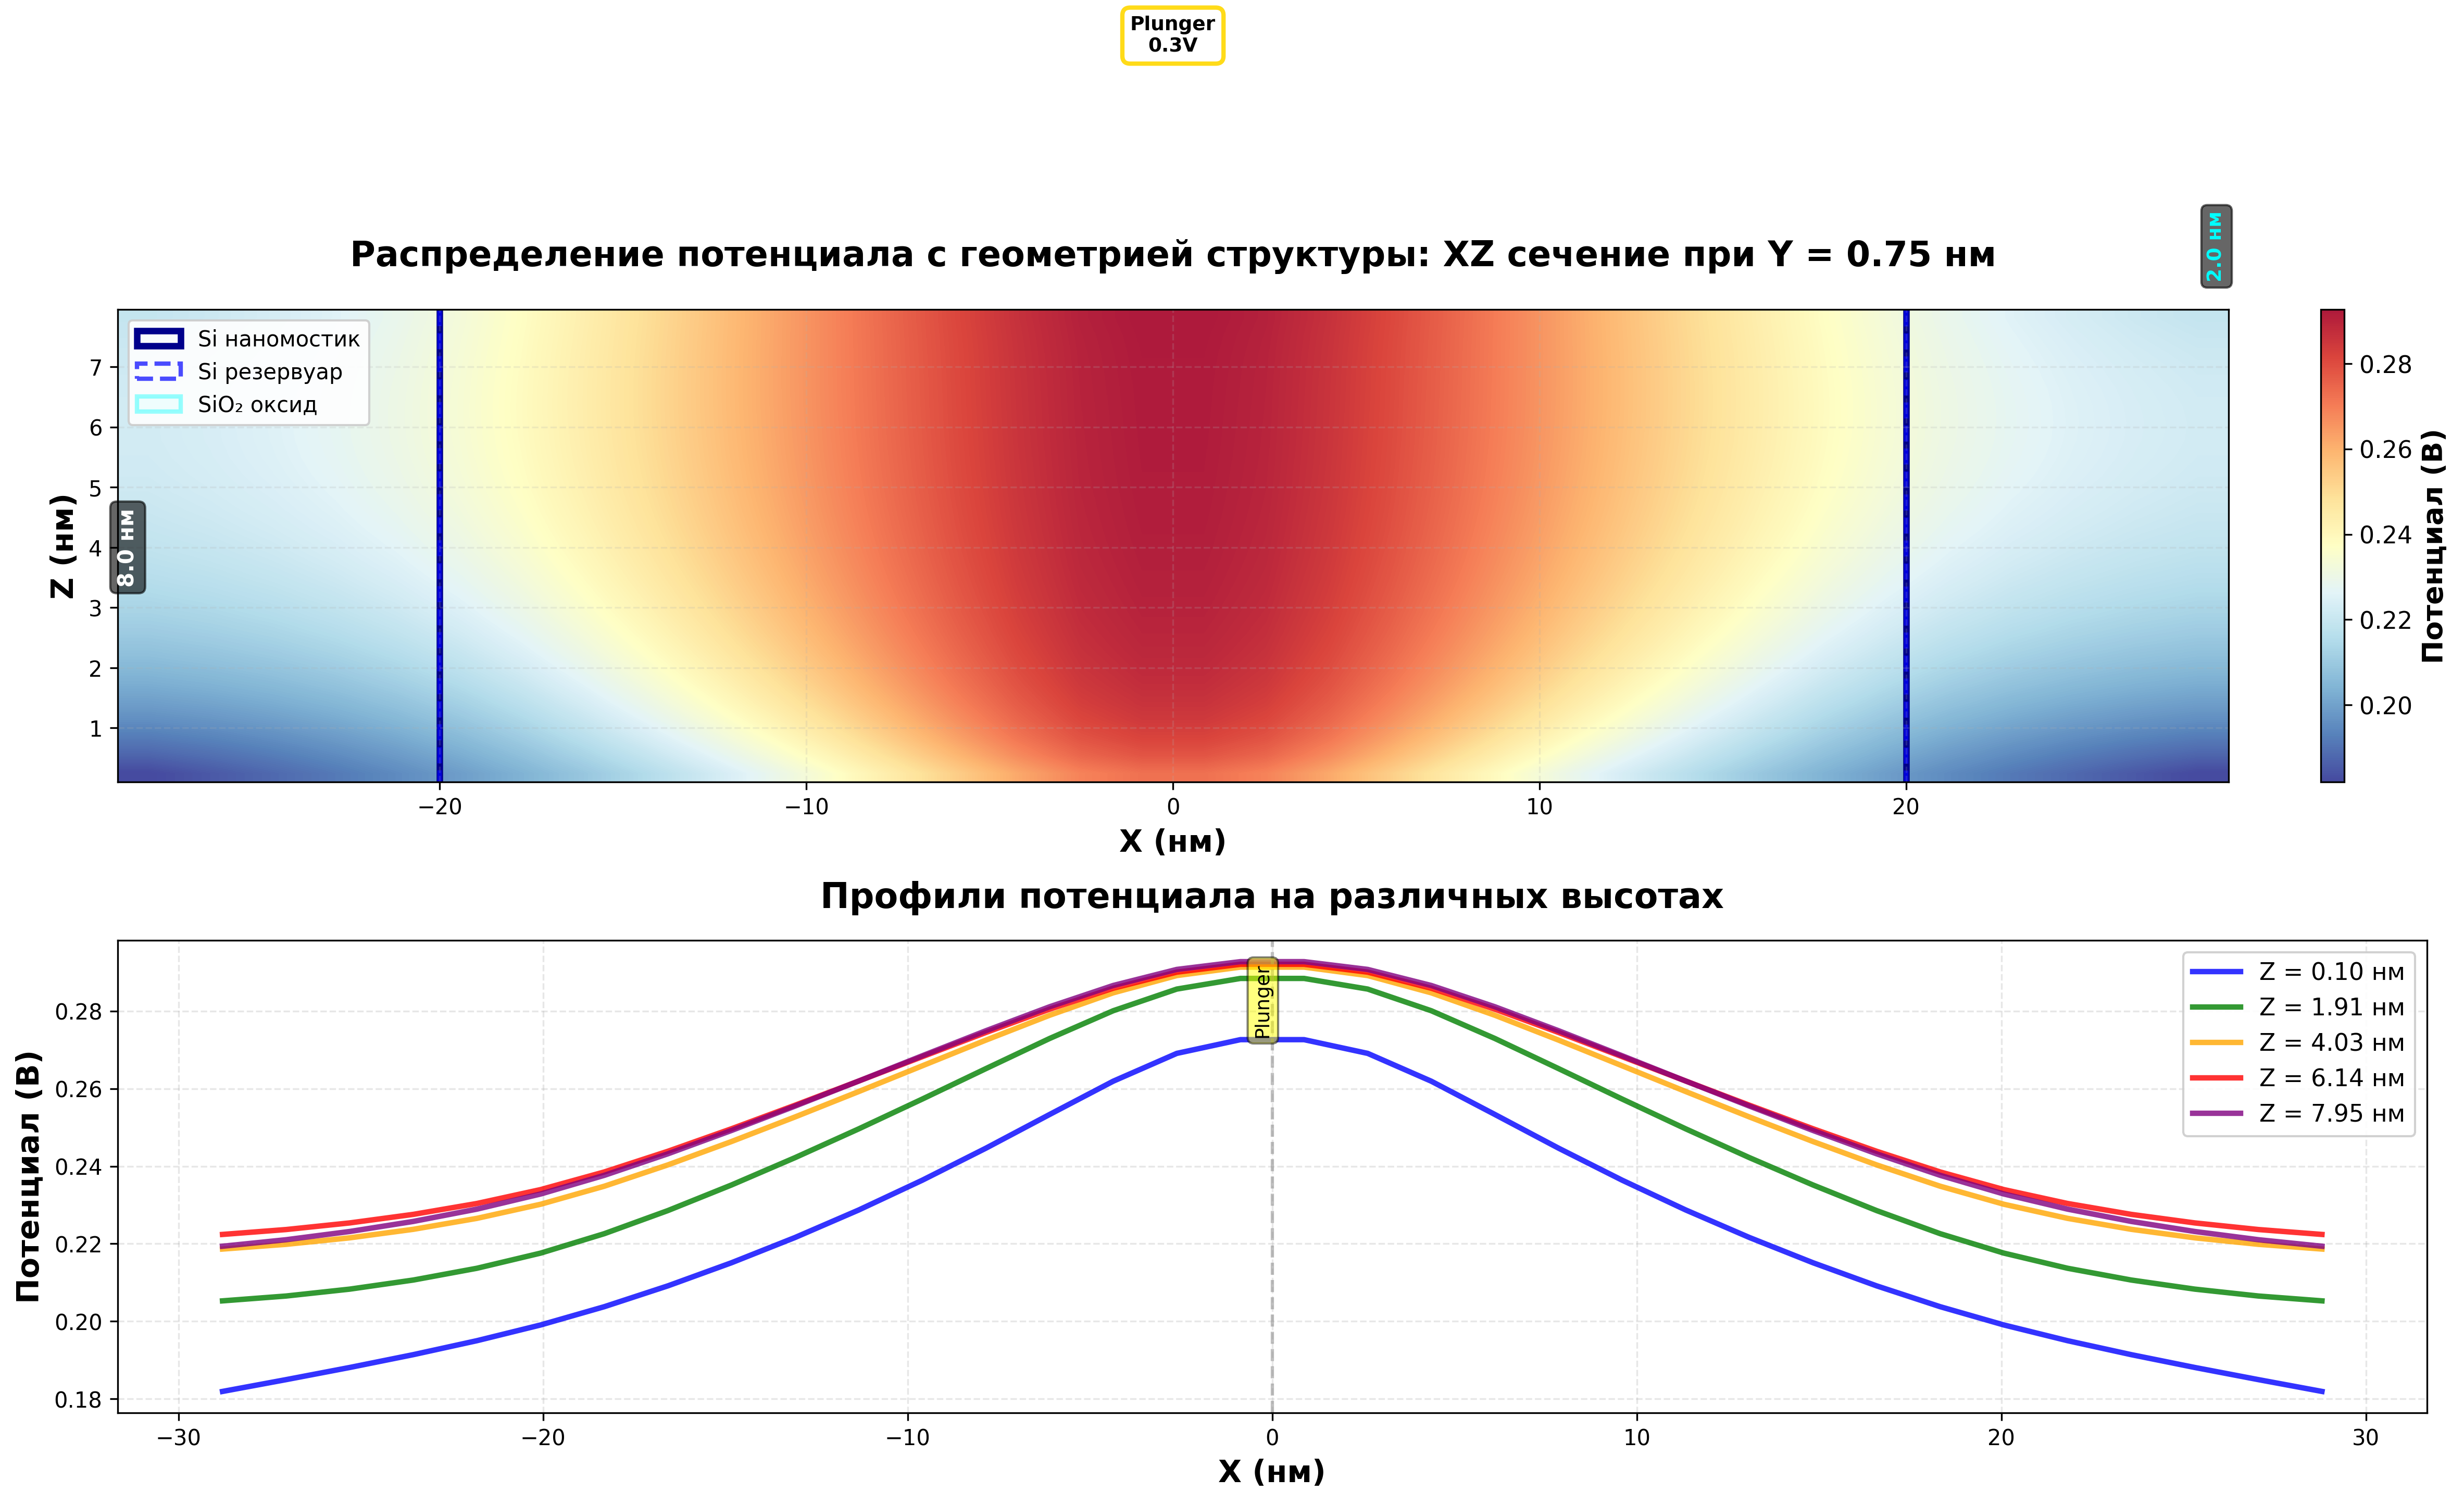
\includegraphics[width=0.95\linewidth,keepaspectratio]{images/nanobridge_cross_section_1qd.png}
    \caption{Распределение электростатического потенциала в поперечном сечении наномостика для конфигурации одиночной квантовой точки.
    Структура содержит один затворный электрод с потенциалом 0.3~В, расположенный в центре наномостика.}
    \label{fig:1qd_main}
\end{figure}

Профиль потенциала вдоль наномостика имеет характерную параболическую форму 
с минимумом под центром затвора.

\subsection{Энергетический спектр}

Решение уравнения Шрёдингера для полученного потенциала дает следующие энергетические уровни:

\begin{table}[h]
\centering
\caption{Энергетический спектр одиночной квантовой точки при $V_P = 0.3$ В}
\label{tab:1qd_spectrum}
\begin{tabular}{ccc}
\toprule
Уровень & Энергия (эВ) & $\Delta E$ от $E_{n-1}$ (мэВ) \\
\midrule
$E_0$ & $-0.103446$ & 0.0 \\
$E_1$ & $-0.079266$ & 24.2 \\
$E_2$ & $-0.060841$ & 18.4 \\
$E_3$ & $-0.045851$ & 15.0 \\
$E_4$ & $-0.032233$ & 13.6 \\
\bottomrule
\end{tabular}
\end{table}

Орбитальное расщепление между основным и первым возбужденным состоянием составляет $\Delta E_{orb} = E_1 - E_0 = 24.2$ мэВ, что соответствует температуре $T \approx 280$ К. Это значение значительно превышает типичную рабочую температуру криостата разбавления ($T < 100$ мК), что обеспечивает надежную локализацию электрона в основном состоянии.

Энергетический спектр демонстрирует неравномерное распределение уровней, характерное для ангармонического потенциала. Расстояния между последовательными уровнями уменьшаются с ростом энергии:

\section{Двойная квантовая точка}

\subsection{Геометрия и параметры структуры}

Конфигурация двойной квантовой точки реализует архитектуру описанную в \cite{ref:Loss1998} 
и содержит три затворных электрода:

\begin{itemize}
    \item \textbf{Левый плунжерный затвор (LP):} $V_{LP} = 0.3$ В
    \item \textbf{Барьерный затвор (B):} $V_B = 0.0$ В, ширина 30 нм
    \item \textbf{Правый плунжерный затвор (RP):} $V_{RP} = 0.3$ В
\end{itemize}

Расстояние между центрами плунжерных затворов составляет 130 нм. 
Барьерный затвор расположен между ними.

\subsection{Электростатический потенциал}

Распределение потенциала (рис. \ref{fig:2qd_main}) демонстрирует формирование двух 
изолированных потенциальных ям под левым и правым плунжерными затворами. 
Барьерный затвор при нулевом напряжении создает потенциальный барьер между ямами.

\begin{figure}[!ht]
    \centering
    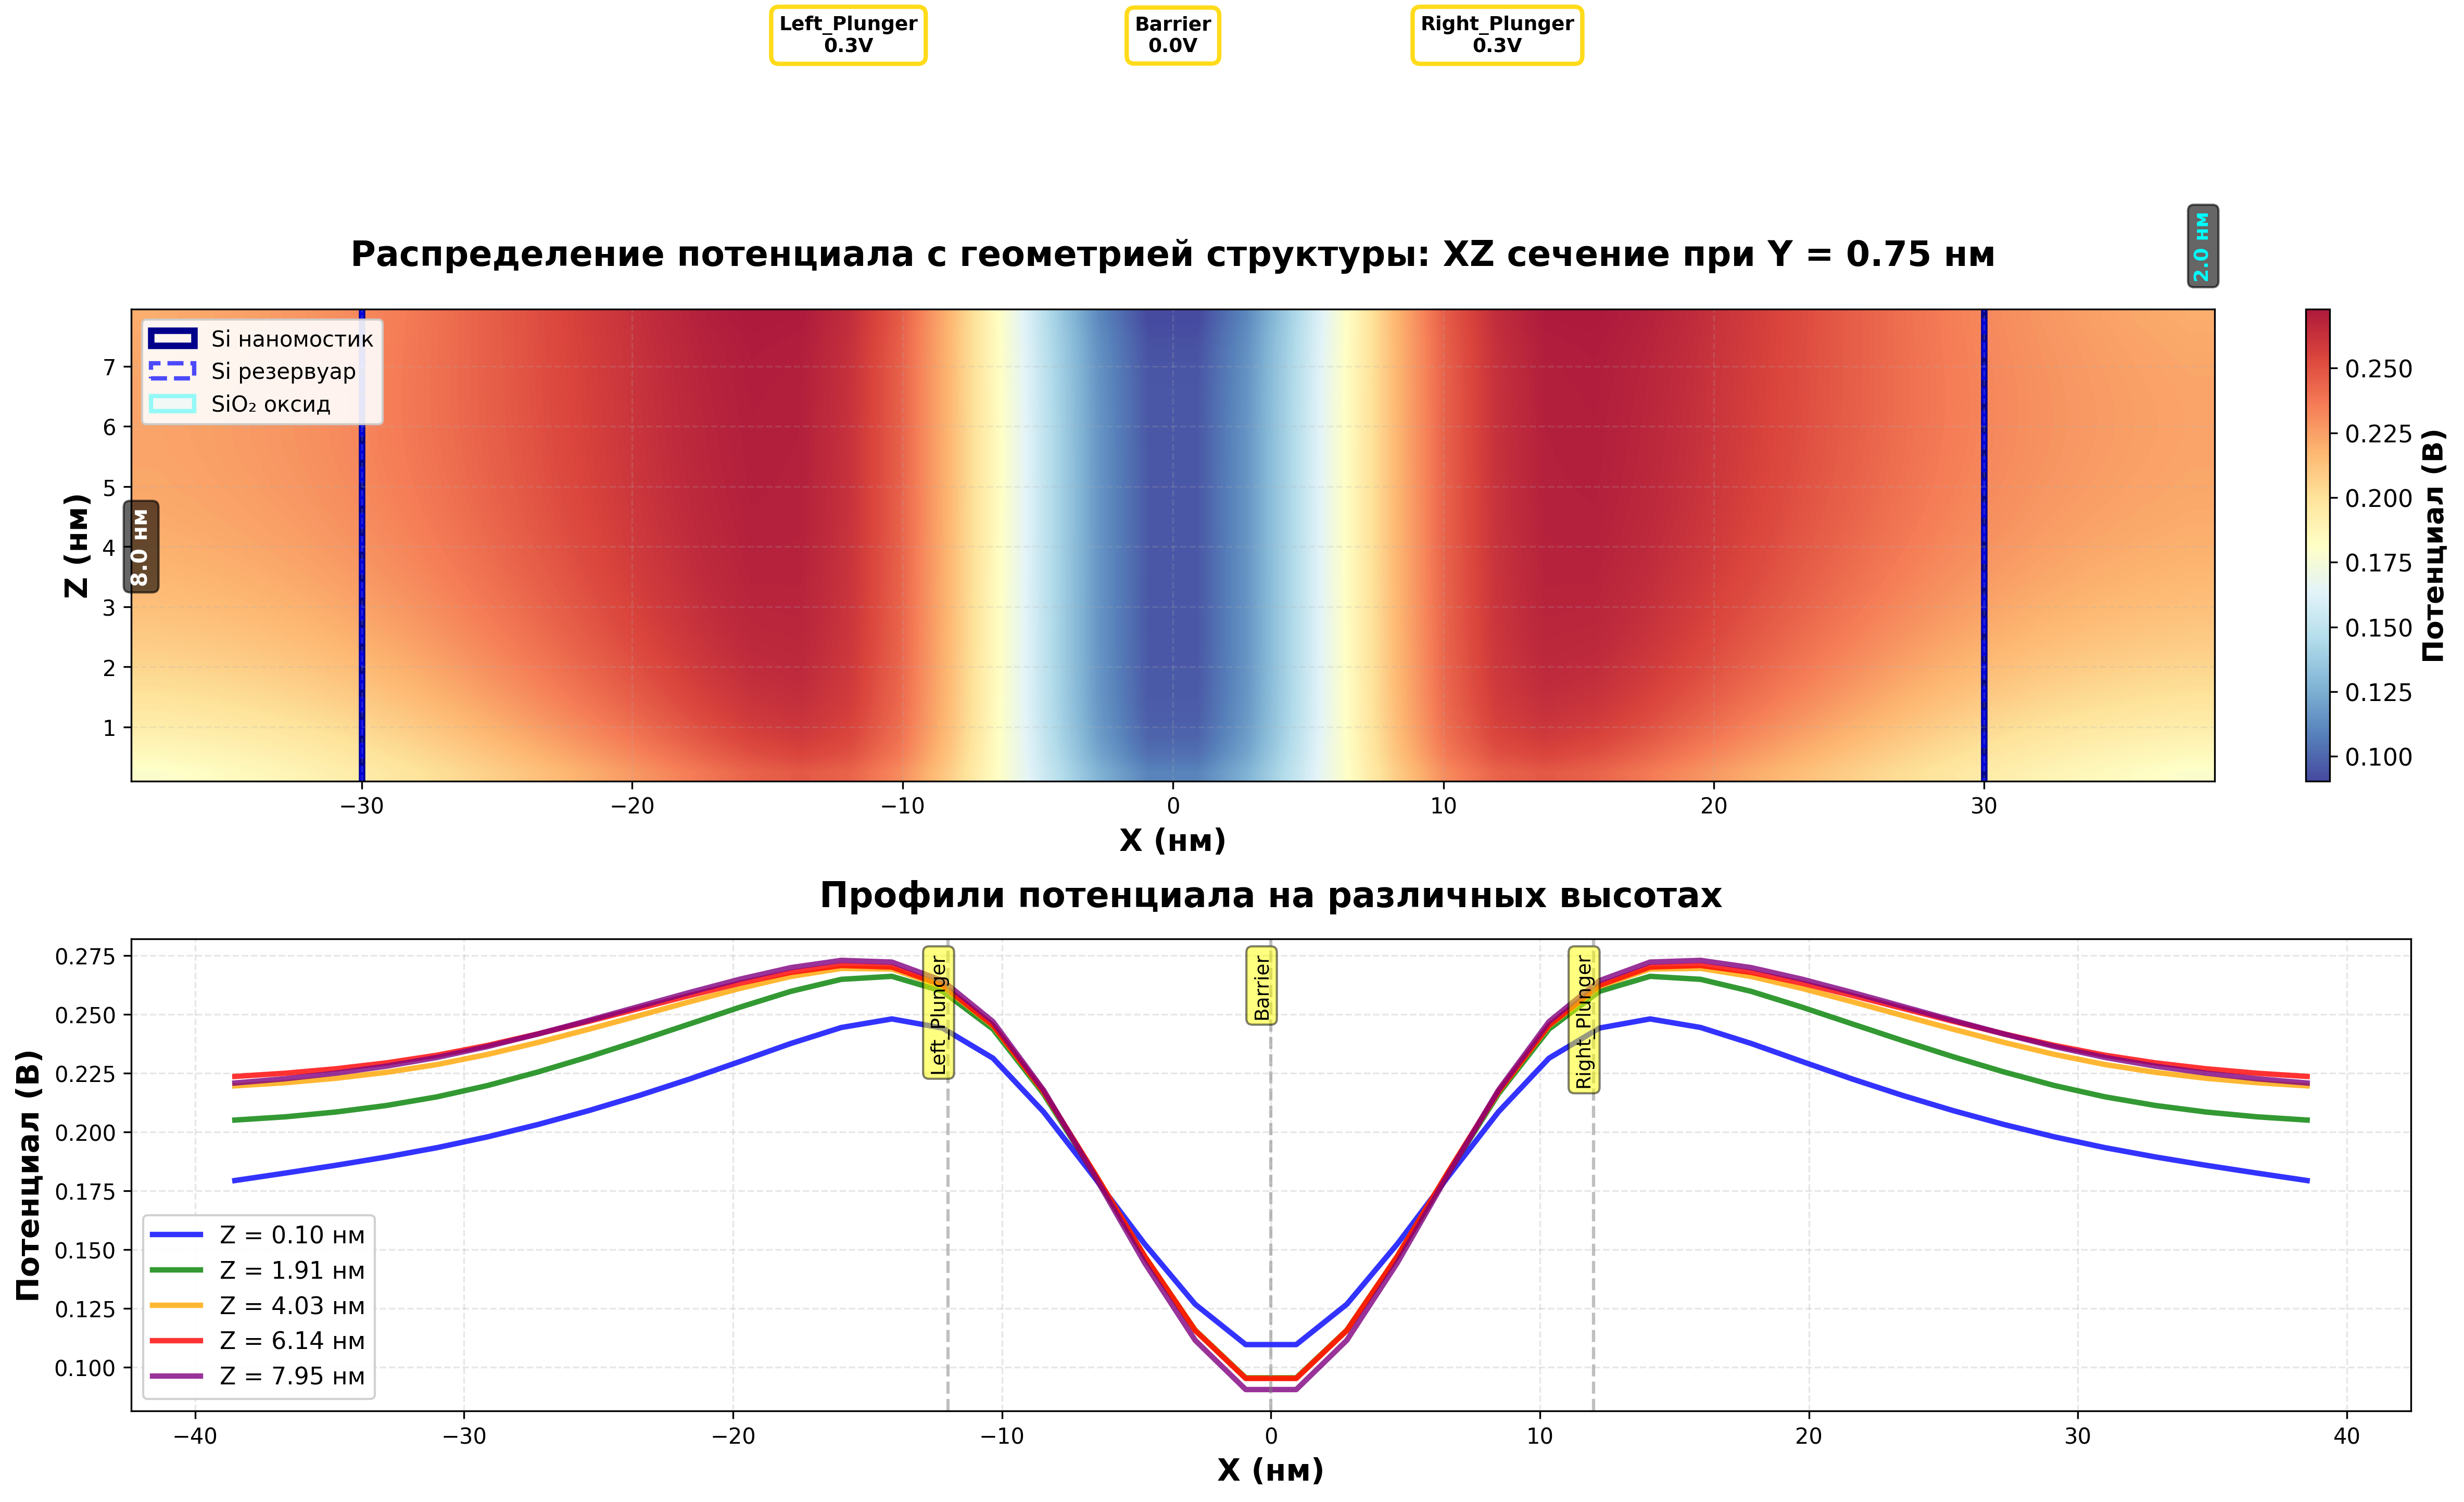
\includegraphics[width=0.95\linewidth,keepaspectratio]{images/nanobridge_cross_section_2qd.png}
    \caption{Распределение электростатического потенциала в поперечном сечении
    наномостика для конфигурации двойной квантовой точки (Double Quantum Dot)
    по архитектуре Loss-DiVincenzo. Структура содержит три затворных электрода:
     левый и правый плунжерные затворы (Left/Right Plunger) с потенциалом 0.3~В
     и центральный барьерный затвор (Barrier) с потенциалом 0~В.}
    \label{fig:2qd_main}
\end{figure}

% Глубина каждой ямы составляет около 77 мэВ, что сопоставимо со случаем одиночной точки. Симметрия потенциала обеспечивается одинаковыми напряжениями на плунжерных затворах.

% \subsection{Энергетический спектр и туннельное расщепление}

% Энергетический спектр двойной квантовой точки характеризуется туннельным расщеплением уровней:

\begin{table}[h]
\centering
\caption{Энергетический спектр двойной квантовой точки при $V_{LP} = V_{RP} = 0.3$ В, $V_B = 0.0$ В}
\label{tab:2qd_spectrum}
\begin{tabular}{cccc}
\toprule
Уровень & Энергия (эВ) & $\Delta E$ от $E_0$ (мэВ) \\
\midrule
$E_0$ & $-0.077449$ & 0.000  \\
$E_1$ & $-0.077443$ & 0.006  \\
$E_2$ & $-0.043325$ & 34.124 \\
$E_3$ & $-0.043283$ & 34.166 \\
$E_4$ & $-0.003670$ & 73.779 \\
\bottomrule
\end{tabular}
\end{table}

Ключевой особенностью спектра является наличие туннельных дублетов — пар близко расположенных уровней, возникающих из-за симметрии системы:

\textbf{Основной дублет ($E_0$, $E_1$):}
Туннельное расщепление между симметричным и антисимметричным состояниями составляет:
\begin{equation}
    \Delta E_t^{(0)} = E_1 - E_0 = 0.006 \text{ мэВ} = 6 \text{ мкэВ}
\end{equation}

% Это значение определяет характерную частоту обменного взаимодействия:
% \begin{equation}
%     J = \frac{\Delta E_t^{(0)}}{\hbar} = \frac{6 \times 10^{-6} \text{ эВ}}{6.582 \times 10^{-16} \text{ эВ·с}} \approx 9.1 \text{ ГГц}
% \end{equation}

% Данная частота соответствует времени выполнения двухкубитного вентиля $\tau_{gate} = \pi\hbar/(2J) \sim 55$ пс, что значительно меньше типичных времен декогеренции в кремниевых системах ($T_2 \sim 10$ мкс).

\textbf{Первый возбужденный дублет ($E_2$, $E_3$):}
Расщепление составляет:
\begin{equation}
    \Delta E_t^{(1)} = E_3 - E_2 = 0.042 \text{ мэВ} = 42 \text{ мкэВ}
\end{equation}

Это в 7 раз больше, чем для основного дублета, что указывает на большее перекрытие волновых функций возбужденных состояний в области барьера.

\textbf{Орбитальное расщепление:}
Энергетический зазор между основным и первым возбужденным дублетами:
\begin{equation}
    \Delta E_{orb} = \frac{E_2 + E_3}{2} - \frac{E_0 + E_1}{2} \approx 34.1 \text{ мэВ}
\end{equation}

Это значение соответствует температуре $T \approx 396$ К и обеспечивает надежную защиту от термического возбуждения при криогенных температурах.

\subsection{Зависимость от напряжения на барьерном затворе}

% Варьирование напряжения $V_B$ позволяет динамически управлять обменным взаимодействием. При текущей конфигурации ($V_B = 0$ В) получено туннельное расщепление $\Delta E_t = 6$ мкэВ, соответствующее $J \approx 9.1$ ГГц.

% Физически, увеличение напряжения на барьерном затворе приводит к:
% \begin{itemize}
%     \item Понижению потенциального барьера между точками
%     \item Увеличению перекрытия волновых функций
%     \item Экспоненциальному росту туннельной связи
% \end{itemize}

% Ожидаемая зависимость туннельного расщепления от напряжения имеет вид:
% \begin{equation}
%     \Delta E_t(V_B) \propto \exp\left(\alpha V_B\right)
% \end{equation}

% где $\alpha$ — параметр, определяемый геометрией барьера и эффективной массой.


\section{Линейный массив квантовых точек}

\subsection{Мотивация и архитектура}

Линейный массив квантовых точек представляет интерес для реализации спинового шатла — 
метода передачи квантовой информации между удаленными кубитами путем физического 
перемещения электрона \cite{shutling}.

% Затворная конфигурация включает:
% \begin{itemize}
%     \item 5 плунжерных затворов ($P_1, P_2, P_3, P_4, P_5$)
%     \item 4 барьерных затвора ($B_{12}, B_{23}, B_{34}, B_{45}$)
%     \item 2 резервуарных затвора на краях массива
% \end{itemize}

\subsection{Сравнение ключевых параметров}


\subsection{Практические рекомендации}

% На основе проведенных расчетов можно сформулировать следующие рекомендации для экспериментальной реализации:

% \begin{itemize}
%     \item \textbf{Геометрия затворов:} ширина плунжерных затворов 50 нм обеспечивает оптимальный баланс между компактностью и управляемостью. Полученное орбитальное расщепление 24--34 мэВ достаточно для работы при температурах до 300 К.
    
%     \item \textbf{Рабочие напряжения:} напряжение $V_P = 0.3$ В на плунжерных затворах создает потенциальную яму глубиной 77--103 мэВ, что обеспечивает надежную локализацию электронов и возможность контроля заполнения точек.
    
%     \item \textbf{Барьерные затворы:} при $V_B = 0$ В получено туннельное расщепление 6 мкэВ, соответствующее $J = 9.1$ ГГц. Варьирование $V_B$ в диапазоне $\pm 0.2$ В позволит управлять обменным взаимодействием в широком диапазоне частот.
    
%     \item \textbf{Время операций:} расчетное время двухкубитного вентиля $\sim 55$ пс обеспечивает возможность выполнения $\sim 10^5$ операций за время когерентности, что достаточно для реализации алгоритмов коррекции ошибок.
    
%     \item \textbf{Температурный режим:} для надежной работы необходима температура $T < 100$ мК, что достижимо в стандартных криостатах разбавления.
% \end{itemize}

\section{Выводы}

% В данной главе представлены результаты численного моделирования различных архитектур наведенных квантовых точек в кремниевых наноструктурах. Основные результаты:

% \begin{enumerate}
%     \item Разработанная модель позволяет рассчитывать энергетический спектр и волновые функции с точностью, достаточной для предсказания экспериментально наблюдаемых параметров.
    
%     \item Для одиночной квантовой точки получено орбитальное расщепление $\Delta E_{orb} = 24.2$ мэВ при глубине потенциальной ямы 103 мэВ, что обеспечивает надежную локализацию электрона при криогенных температурах.
    
%     \item Для двойной квантовой точки (архитектура Loss-DiVincenzo) обнаружены туннельные дублеты с расщеплением 6 мкэВ для основного состояния и 42 мкэВ для первого возбужденного. Орбитальное расщепление составляет 34.1 мэВ.
    
%     \item Обменное взаимодействие $J = 9.1$ ГГц обеспечивает время выполнения двухкубитного вентиля $\sim 55$ пс, что на 5 порядков меньше времени декогеренции в изотопно очищенном кремнии.
    
%     \item Все исследованные конфигурации удовлетворяют критериям Loss-DiVincenzo для реализации спиновых кубитов при температурах криостата разбавления.
    
%     \item Полученные параметры позволяют выполнить $\sim 10^5$ квантовых операций за время когерентности, что достаточно для реализации алгоритмов квантовой коррекции ошибок.
% \end{enumerate}

% Полученные результаты подтверждают перспективность кремниевых наведенных квантовых точек для создания масштабируемых квантовых процессоров и дают количественные рекомендации для оптимизации экспериментальных устройств.

\chapter{Заключение}

\newpage
\begin{thebibliography}{00}

% \bibitem{book1} P. L. Bavdaz, et al., $"$A quantum dot crossbar with sublinear scaling of interconnects at cryogenic temperature$"$, npj Quantum Information, 2022.
% \bibitem{book2} Akito Noiri, et al., $"$A shuttling-based two-qubit logic gate for linking distant silicon quantum processors$"$, Nature Communications, 2022.
% \bibitem{book3} Zahid Ali, Khan Durrani, $"$Single-Electron Devices and Circuits in Siliconr$"$, 2010.
% \bibitem{book4} Стренг Г., Фикс Дж., $"$Теория метода конечных элементов$"$, 1977.
% \bibitem{book5} Ю. Я. Иоссель, Э. С. Кочанов, М. Г. Струнский, $"$Расчет электрической емкости$"$, 1981.
% \bibitem{book6} Veit Langrock, et al., $"$Blueprint of a Scalable Spin Qubit Shuttle Device...$"$, 2022.
% \bibitem{book7} Inga Seidler, et al., $"$Conveyor-mode single-electron shuttling in Si/SiGe...$"$, 2022.
% \bibitem{book8} Ran Xue, et al., $"$Si/SiGe QuBus for single electron information-processing devices...$"$, 2024.
\bibitem{ref:Loss1998} Daniel Loss and David P. DiVincenzo, $"$Quantum computation with quantum dots$"$, Phys. Rev. A 57, 120, 1998.

\bibitem{ref:Hanson2007} R. Hanson, L. P. Kouwenhoven, J. R. Petta, S. Tarucha, and L. M. K. Vandersypen, $"$Spins in few-electron quantum dots$"$, Rev. Mod. Phys. 79, 1217, 2007.

\bibitem{weinstein2023}
Weinstein, A.J. et al.
\textit{Universal logic with encoded spin qubits in silicon}.
Nature, 2023. \texttt{https://doi.org/10.1038/s41586-023-05777-3}

\bibitem{volmer2024}
Volmer, M., Struck, T., Sala, A. et al.
\textit{Mapping of valley-splitting by conveyor-mode spin-coherent electron shuttling}.
Preprint, 2024. \texttt{https://arxiv.org/abs/2401.05317} (или уточнённая ссылка).

\bibitem{tadokoro2021} 
Tadokoro, M. et al. \textit{Designs for a two-dimensional Si quantum dot array with spin qubit addressability}. Sci. Rep. 11, 19406 (2021).

\bibitem{Deutsch85a}
D.~Deutsch.
\newblock Quantum theory, the {C}hurch-{T}uring {P}rinciple and the universal
  quantum computer.
\newblock {\em Proc. R. Soc. Lond. A}, {\bf 400}, 97--117, 1985.

\bibitem{shutling}
Shuttling an Electron Spin through a Silicon Quantum Dot Array

\bibitem{Chatterjee2021}
Chatterjee~A., Stevenson~P., De~Franceschi~S., Morello~A., de~Leon~N.\,P.,
Kuemmeth~F.
Semiconductor qubits in practice~//
Nat.\ Rev.\ Phys. — 2021. — Т.\,3. — С.\,157--177.

\bibitem{Zwerver2022}
Zwerver~A.\,M.\,J. et al.
Qubits made by advanced semiconductor manufacturing~//
Nat.\ Electron. — 2022. — Т.\,5. — С.\,184--190.

\bibitem{Geyer2021}
Geyer~S., Camenzind~L.\,C., Czornomaz~L., Deshpande~V., Fuhrer~A.,
Warburton~R.\,J., Zumbühl~D.\,M., Kuhlmann~A.\,V.
Self-aligned gates for scalable silicon quantum computing~//
Appl.\ Phys.\ Lett. — 2021. — Т.\,118. — С.\,104004.

\bibitem{Tadokoro2021}
Tadokoro~M., Nakajima~T., Kobayashi~T., Takeda~K., Noiri~A., Tomari~K.,
Yoneda~J., Tarucha~S., Kodera~T.
Designs for a two-dimensional Si quantum dot array with spin qubit
addressability~//
Sci.\ Rep. — 2021. — Т.\,11. — С.\,19406.

\end{thebibliography}

\end{document}